% !Mode:: "TeX:UTF-8"
\chapter{视觉里程计1}
\label{cpt:7}
\thispagestyle{empty}

\begin{mdframed}  
	\textbf{主要目标}
	\begin{enumerate}[labelindent=0em,leftmargin=1.5em]
		\item 理解图像特征点的意义, 并掌握在单幅图像中提取出特征点及多幅图像中匹配特征点的方法。
		\item 理解对极几何的原理,利用对极几何的约束,恢复出图像之间的摄像机的三维运动。
		\item 理解PNP问题,以及利用已知三维结构与图像的对应关系求解摄像机的三维运动。
		\item 理解ICP问题,以及利用点云的匹配关系求解摄像机的三维运动。
		\item 理解如何通过三角化获得二维图像上对应点的三维结构。
	\end{enumerate}
\end{mdframed}

本书前面介绍了运动方程和观测方程的具体形式,并讲解了以非线性优化为主的求解方法。从本讲开始,我们结束基础知识的铺垫而步入正题:按照第2讲的顺序,分别介绍视觉里程计、优化后端、回环检测和地图构建4个模块。本讲和下一讲主要介绍两类视觉里程计里常用的方法:特征点法和光流法。本讲中,我们将介绍什么是特征点、如何提取和匹配特征点,以及如何根据配对的特征点估计相机运动。

\newpage
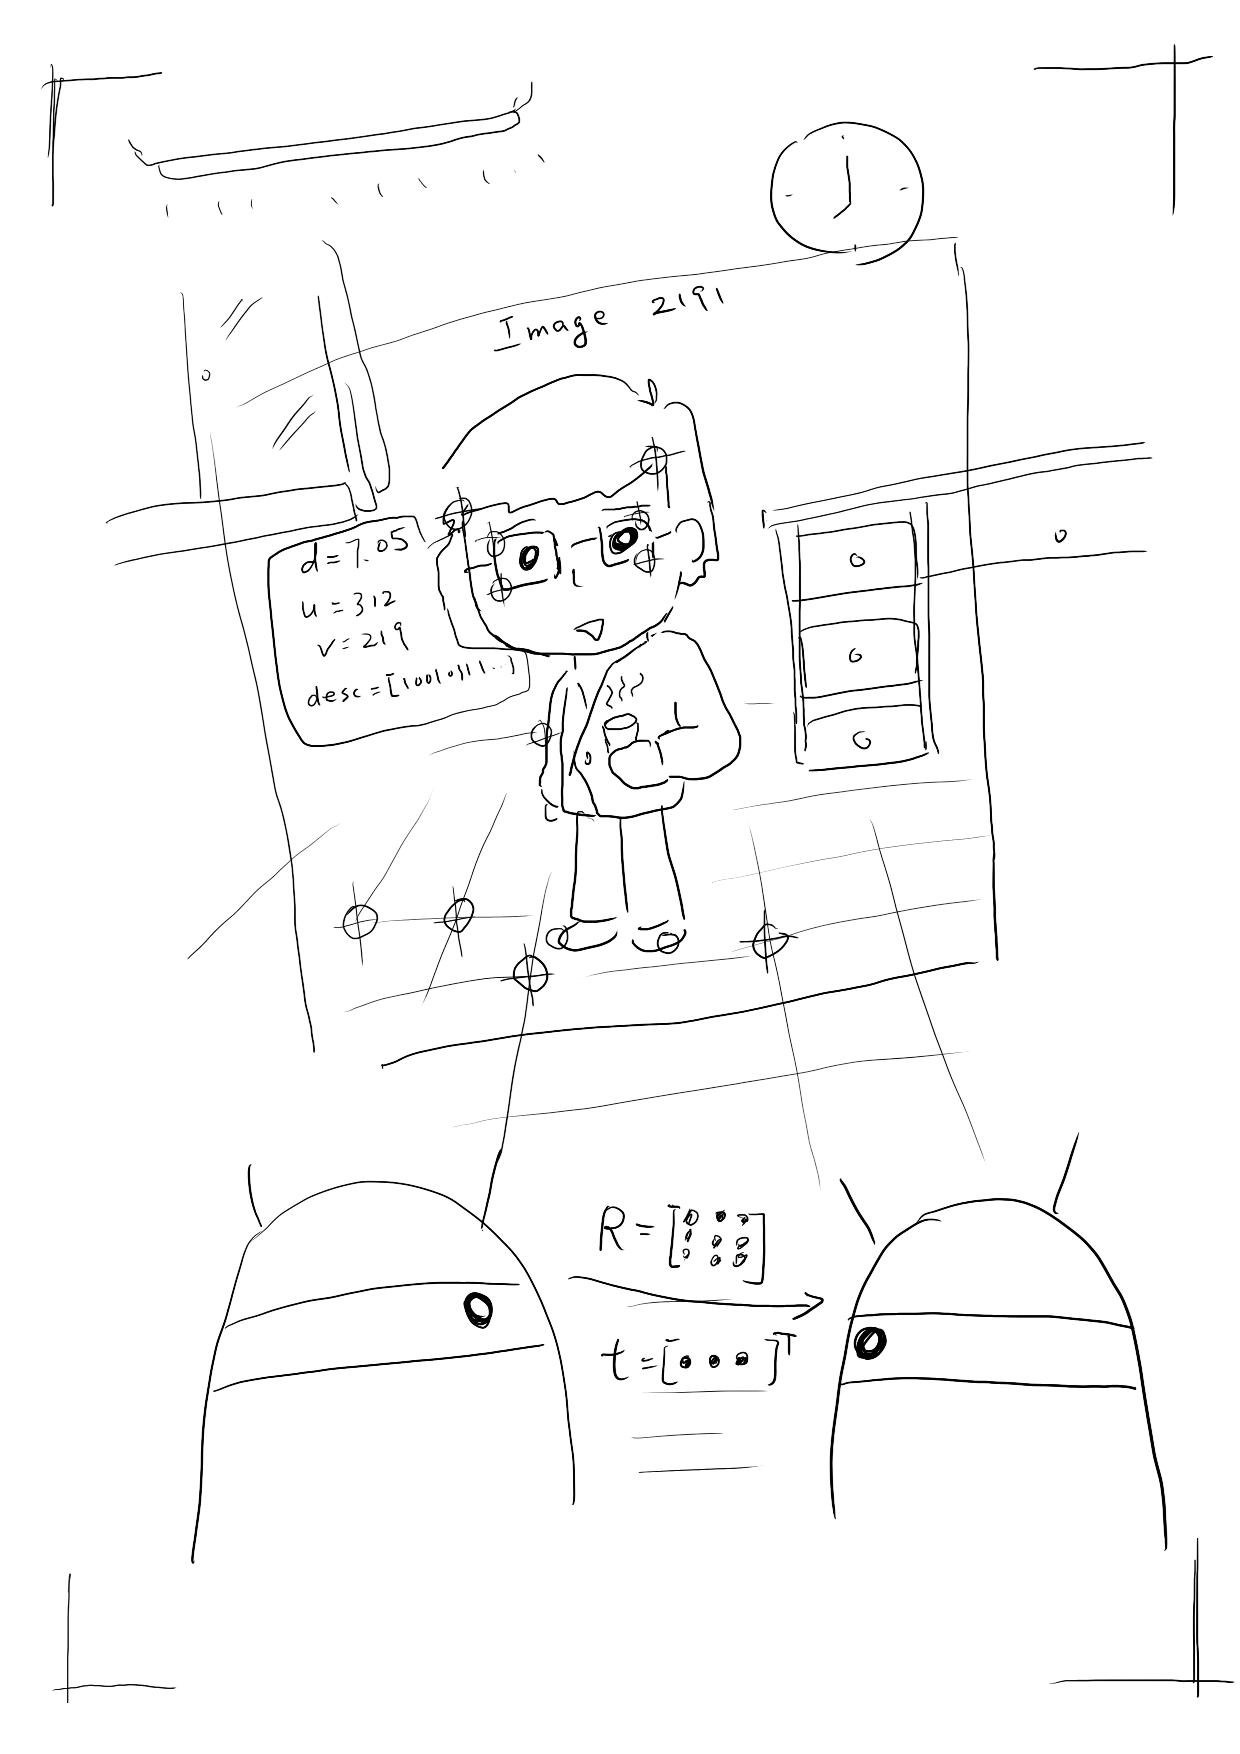
\includepdf{resources/other/ch7.pdf}

\newpage

\section{特征点法}
在第二讲中,我们说,一个SLAM系统分为前端和后端,其中前端也称为视觉里程计(VO)。VO根据相邻图像的信息估计出粗略的相机运动,给后端提供较好的初始值。VO的算法主要分为两个大类:\textbf{特征点法}和\textbf{直接法}。基于特征点法的前端,长久以来(直到现在)被认为是视觉里程计的主流方法。它具有稳定,对光照、动态物体不敏感的优势,是目前比较成熟的解决方案。在本讲中,我们将从特征点法入手,学习如何提取、匹配图像特征点,然后估计两帧之间的相机运动和场景结构,从而实现一个两帧间视觉里程计。这类算法有时也称为两视图几何(Two-view geometry)。

\subsection{特征点}
VO的核心问题是\textbf{如何根据图像来估计相机运动}。然而,图像本身是一个由亮度和色彩组成的矩阵,如果直接从矩阵层面考虑运动估计,将会非常困难。所以,比较方便的做法是:首先,从图像中选取比较\textbf{有代表性}的\textbf{点}。这些点在相机视角发生少量变化后会保持不变,于是我们能在各个图像中找到相同的点。然后,在这些点的基础上,讨论相机位姿估计问题,以及这些点的定位问题。在经典SLAM模型中,我们称这些点为\textbf{路标}(Landmark)。而在视觉SLAM中,路标则是指图像特征(Feature)。

根据维基百科的定义,图像特征是一组与计算任务相关的信息,计算任务取决于具体的应用\textsuperscript{\cite{wiki:featurecv}}。简而言之,\textbf{特征是图像信息的另一种数字表达形式}。一组好的特征对于在指定任务上的最终表现至关重要,所以多年来研究者们花费了大量的精力对特征进行研究。数字图像在计算机中以灰度值矩阵的方式存储,所以最简单的,单个图像像素也是一种“特征”。但是,在视觉里程计中,我们希望\textbf{特征点在相机运动之后保持稳定},而灰度值受光照、形变、物体材质的影响严重,在不同图像间变化非常大,不够稳定。理想的情况是,当场景和相机视角发生少量改变时,算法还能从图像中判断哪些地方是同一个点。所以,仅凭灰度值是不够的,我们需要对图像提取特征点。

特征点是图像里一些\textbf{特别的地方}。以\autoref{fig:corner-feature}~为例。我们可以把图像中的角点、边缘和区块都当成图像中有代表性的地方。不过,我们更容易精确地指出,某两幅图像中出现了同一个角点;同一个边缘则稍微困难一些,因为沿着该边缘前进,图像局部是相似的;同一个区块则是最困难的。我们发现,图像中的角点、边缘相比于像素区块而言更加“特别”,在不同图像之间的辨识度更强。所以,一种直观的提取特征的方式就是在不同图像间辨认角点,确定它们的对应关系。在这种做法中,角点就是所谓的特征。角点的提取算法有很多,例如Harris角点\textsuperscript{\cite{Harris1988}}、FAST角点\textsuperscript{\cite{Rosten2006}}、GFTT角点\textsuperscript{\cite{Shi1994}},等等。它们大部分是2000年以前提出的算法。

然而,在大多数应用中,单纯的角点依然不能满足我们的很多需求。例如,从远处看上去是角点的地方,当相机走近之后,可能就不显示为角点了。或者,当旋转相机时,角点的外观会发生变化,我们也就不容易辨认出那是同一个角点。为此,计算机视觉领域的研究者们在长年的研究中设计了许多更加稳定的局部图像特征,如著名的SIFT\textsuperscript{\cite{Lowe2004}}、SURF\textsuperscript{\cite{Bay2006}}、ORB\textsuperscript{\cite{Rublee2011}},等等。相比于朴素的角点,这些人工设计的特征点能够拥有如下的性质:

\begin{enumerate}
\item \emph{可重复性}(Repeatability):相同的特征可以在不同的图像中找到。
\item \emph{可区别性}(Distinctiveness):不同的特征有不同的表达。
\item \emph{高效率}(Efficiency):同一图像中,特征点的数量应远小于像素的数量。
\item \emph{本地性}(Locality):特征仅与一小片图像区域相关。
\end{enumerate}

\begin{figure}[!ht]
    \centering
    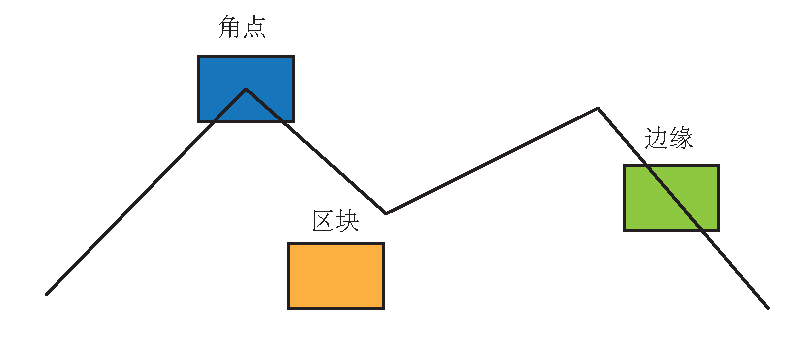
\includegraphics[width=0.8\linewidth]{vo1/corner-flat-line}\\
    \caption{可以作为图像特征的部分:角点、边缘、区块。}
    \label{fig:corner-feature}
\end{figure}

特征点由\textbf{关键点}(Key-point)和\textbf{描述子}(Descriptor)两部分组成。比如,当我们说“在一张图像中计算SIFT特征点”,是指“提取SIFT关键点,并计算SIFT描述子”两件事情。关键点是指该特征点在图像里的位置,有些特征点还具有朝向、大小等信息。描述子通常是一个向量,按照某种人为设计的方式,描述了该关键点周围像素的信息。描述子是按照“\textbf{外观相似的特征应该有相似的描述子}”的原则设计的。因此,只要两个特征点的描述子在向量空间上的距离相近,就可以认为它们是同样的特征点。

历史上,研究者们提出过许多图像特征。它们有些很精确,在相机的运动和光照变化下仍具有相似的表达,但相应地需要较大的计算量。其中,SIFT(尺度不变特征变换,Scale-Invariant Feature Transform)当属最为经典的一种。它充分考虑了在图像变换过程中出现的光照、尺度、旋转等变化,但随之而来的是极大的计算量。由于整个SLAM过程中图像特征的提取与匹配仅仅是诸多环节中的一个,到目前(2016年)为止,普通PC的CPU还无法实时地计算SIFT特征,进行定位与建图\footnote{这里是指30Hz的实时速度。}。所以在SLAM中我们甚少使用这种“奢侈”的图像特征。

另一些特征,则考虑适当降低精度和鲁棒性,以提升计算的速度。例如,FAST关键点属于计算特别快的一种特征点(注意这里“关键点”的表述,说明它没有描述子),而ORB(Oriented FAST and Rotated BRIEF)特征则是目前看来非常具有代表性的实时图像特征。它改进了FAST检测子\textsuperscript{\cite{Rosten2006}}不具有方向性的问题,并采用速度极快的二进制描述子BRIEF\textsuperscript{\cite{calonder2010brief}},使整个图像特征提取的环节大大加速。根据作者在论文中所述测试,在同一幅图像中同时提取约1000个特征点的情况下,ORB约要花费15.3ms,SURF约花费217.3ms,SIFT约花费5228.7ms。由此可以看出,ORB在保持了特征子具有旋转、尺度不变性的同时,速度方面提升明显,对于实时性要求很高的SLAM来说是一个很好的选择。

大部分特征提取都具有较好的并行性,可以通过GPU等设备来加速计算。经过GPU加速后的SIFT,就可以满足实时计算要求。但是,引入GPU将带来整个SLAM成本的提升。由此带来的性能提升是否足以抵去付出的计算成本,需要系统的设计人员仔细考量。

显然,计算机视觉领域存在大量的特征点种类,我们不可能在书中一一介绍。在目前的SLAM方案中,ORB是质量与性能之间较好的折中,因此,我们以ORB为代表介绍提取特征的整个过程。如果读者对特征提取和匹配算法感兴趣,我们建议阅读这方面的相关书籍\cite{Nixon2012}。

\subsection{ORB特征}

ORB特征亦由\textbf{关键点}和\textbf{描述子}两部分组成。它的关键点称为“Oriented FAST”,是一种改进的FAST角点,关于什么是FAST角点我们将在下文介绍。它的描述子称为BRIEF(Binary Robust Independent Elementary Feature)。因此,提取ORB特征分为如下两个步骤:
\begin{enumerate}
\item FAST角点提取:找出图像中的“角点”。相较于原版的FAST,ORB中计算了特征点的主方向,为后续的BRIEF描述子增加了旋转不变特性。
\item BRIEF描述子:对前一步提取出特征点的周围图像区域进行描述。ORB对BRIEF进行了一些改进,主要是指在BRIEF中使用了先前计算的方向信息。
\end{enumerate}

下面分别介绍FAST和BRIEF。
\subsubsection{FAST关键点}

FAST是一种角点,主要检测局部像素灰度变化明显的地方,以速度快著称。它的思想是:如果一个像素与邻域的像素差别较大(过亮或过暗),那么它更可能是角点。相比于其他角点检测算法,FAST只需比较像素亮度的大小,十分快捷。它的检测过程如下(见\autoref{fig:fastcorner}~):

\begin{enumerate}
\item 在图像中选取像素$p$,假设它的亮度为$I_{p}$。
\item 设置一个阈值$T$(比如,$I_{p}$的20\%)。
\item 以像素$p$为中心,选取半径为3的圆上的16个像素点。
\item 假如选取的圆上有连续的$N$个点的亮度大于$I_{p}+T$或小于$I_{p}-T$,那么像素$p$可以被认为是特征点($N$通常取12,即为FAST-12。其他常用的$N$取值为9和11,它们分别被称为FAST-9和FAST-11)。
\item 循环以上四步,对每一个像素执行相同的操作。
\end{enumerate}

在FAST-12算法中,为了更高效,可以添加一项预测试操作,以快速地排除绝大多数不是角点的像素。具体操作为,对于每个像素,直接检测邻域圆上的第1, 5, 9, 13个像素的亮度。只有当这4个像素中有3个同时大于$I_{p}+T$或小于$I_{p}-T$时,当前像素才有可能是一个角点,否则应该直接排除。这样的预测试操作大大加速了角点检测。此外,原始的FAST角点经常出现“扎堆”的现象。所以在第一遍检测之后,还需要用非极大值抑制(Non-maximal suppression),在一定区域内仅保留响应极大值的角点,避免角点集中的问题。

\begin{figure}[!ht]
	\centering
	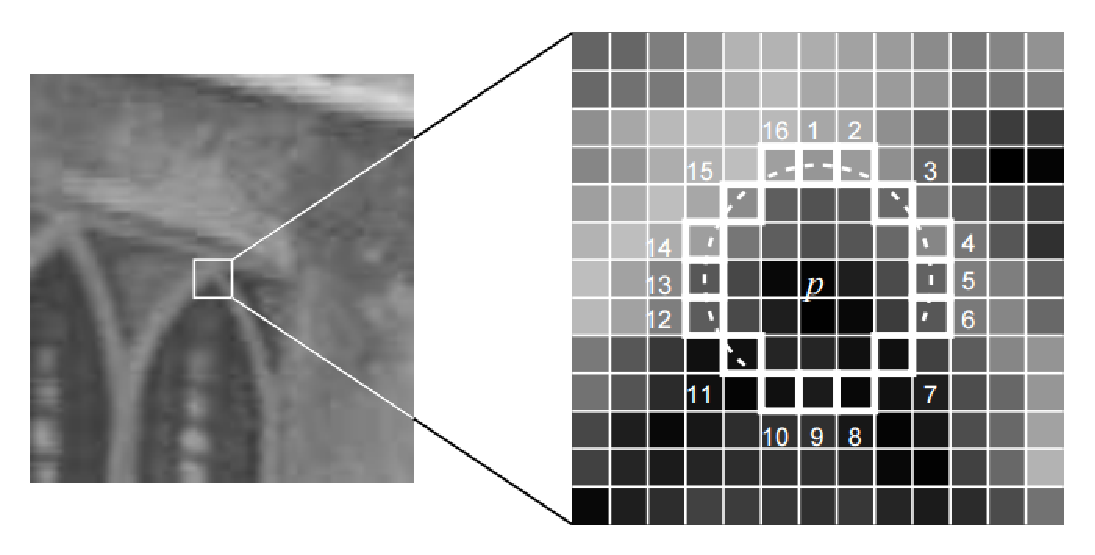
\includegraphics[width=0.9\linewidth]{vo1/fast-corner}
	\caption{FAST特征点\textsuperscript{\cite{Rosten2006}}。}
	\label{fig:fastcorner}
\end{figure}

FAST特征点的计算仅仅是比较像素间亮度的差异所所以速度非常快,但它也有重复性不强,分布不均匀的缺点。此外,FAST角点不具有方向信息。同时,由于它固定取半径为3的圆,存在尺度问题:远处看着像是角点的地方,接近后看可能就不是角点了。针对FAST角点不具有方向性和尺度的弱点,ORB添加了尺度和旋转的描述。尺度不变性由构建图像金字塔\footnote{金字塔是指对图像进行不同层次的降采样,以获得不同分辨率的图像。},并在金字塔的每一层上检测角点来实现。而特征的旋转是由灰度质心法(Intensity Centroid)实现的。

金字塔时计算图视觉中常用的一种处理方法,示意图见\autoref{fig:pyramid}。金字塔底层是原始图像。每往上一层,就对图像进行一个固定倍率的缩放,这样我们就有了不同分辨率的图像。较小的图像可以看成是远处看过来的场景。在特征匹配算法中,我们可以匹配不同层上的图像,从而实现尺度不变性。例如,如果相机在后退,那么我们应该能够在上一个图像金字塔的上层和下一个图像的下层中找到匹配。

\begin{figure}[!t]
    \centering
    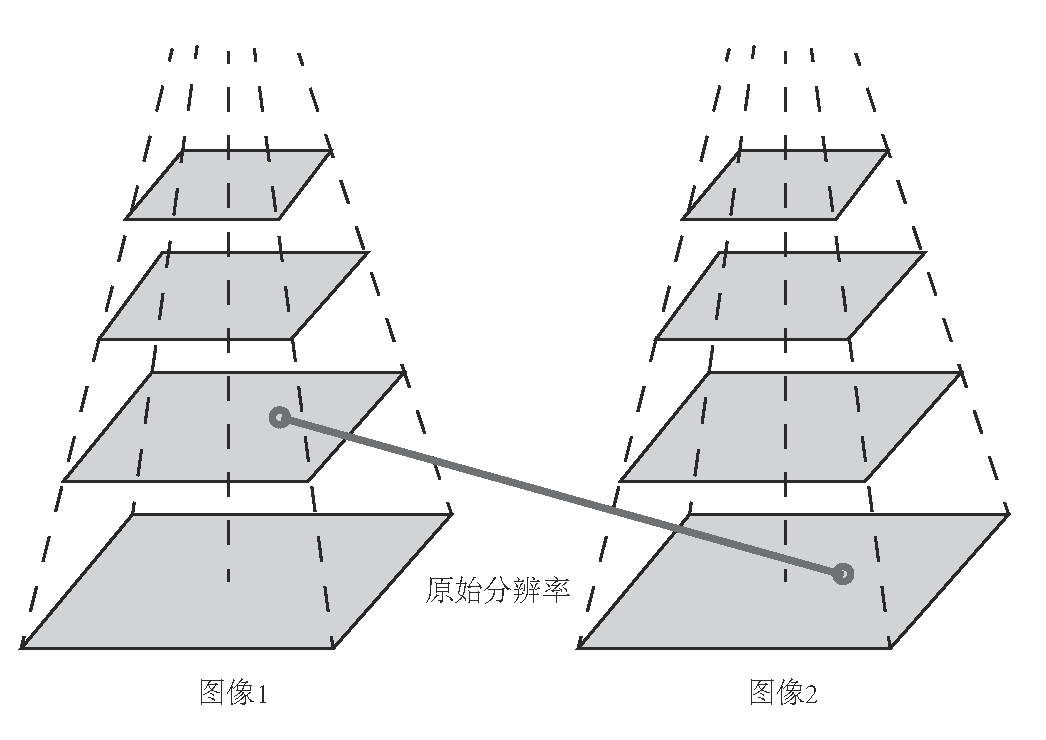
\includegraphics[width=0.9\linewidth]{vo1/pyramid}\\
    \caption{使用金字塔可以匹配不同缩放倍率下的图像。}
    \label{fig:pyramid}
\end{figure}

在旋转方面,我们计算特征点附近的图像灰度质心。所谓质心是指以图像块灰度值作为权重的中心。其具体操作步骤如下\textsuperscript{\cite{Rosin1999}}:
\begin{enumerate}
\item 在一个小的图像块$B$中,定义图像块的矩为
\[
m_{pq}=\sum_{x,y \in B}x^{p}y^{q}I(x,y), \quad p, q = \{0,1\}.
\]
\item 通过矩可以找到图像块的质心:
\[
C=\left(\frac{m_{10}}{m_{00}},\frac{m_{01}}{m_{00}}\right).
\]
\item 连接图像块的几何中心$O$与质心$C$,得到一个方向向量$\overrightarrow{OC}$,于是特征点的方向可以定义为
\[
\theta = \arctan(m_{01}/m_{10}).
\]
\end{enumerate}
通过以上方法,FAST角点便具有了尺度与旋转的描述,从而大大提升了其在不同图像之间表述的鲁棒性。所以在ORB中,把这种改进后的FAST称为Oriented FAST。

\subsubsection{BRIEF描述子}
在提取Oriented FAST关键点后,我们对每个点计算其描述子。ORB使用改进的BRIEF特征描述。我们先来介绍一下BRIEF是什么。

BRIEF是一种\textbf{二进制}描述子,其描述向量由许多个0和1组成,这里的0和1编码了关键点附近两个随机像素(比如$p$和$q$)的大小关系:如果$p$比$q$大,则取1,反之就取0。如果我们取了128个这样的$p,q$,最后就得到128维由0、1组成的向量\textsuperscript{\cite{calonder2010brief}}。BRIEF使用了随机选点的比较,速度非常快,而且由于使用了二进制表达,存储起来也十分方便,适用于实时的图像匹配。原始的BRIEF描述子不具有旋转不变性,因此在图像发生旋转时容易丢失。而ORB在FAST特征点提取阶段计算了关键点的方向,所以可以利用方向信息,计算了旋转之后的“Steer BRIEF”特征使ORB的描述子具有较好的旋转不变性。

由于考虑到了旋转和缩放,使得ORB在平移、旋转和缩放的变换下仍有良好的表现。同时,FAST和BREIF的组合也非常高效,使得ORB特征在实时SLAM中非常受欢迎。我们在\autoref{fig:ORB}~中展示了一张图像提取ORB之后的结果,下面来介绍如何在不同的图像之间进行特征匹配。

\begin{figure}[!htp]
    \centering
    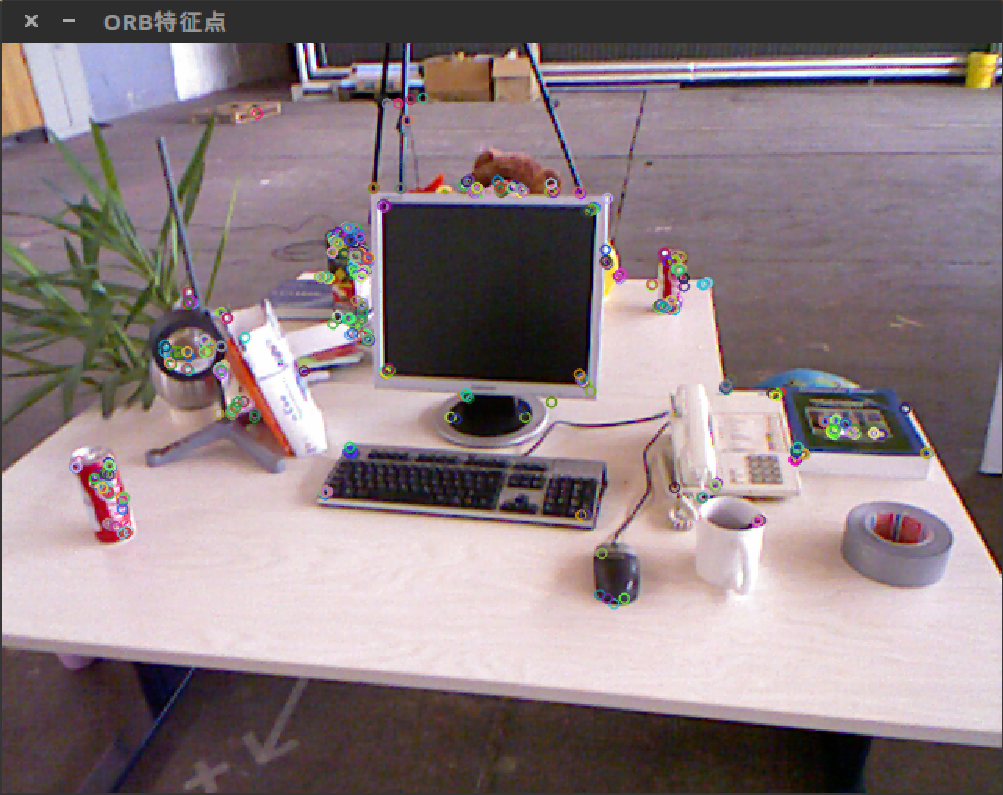
\includegraphics[width=0.9\linewidth]{vo1/feature}\\
    \caption{OpenCV提供的ORB特征点检测结果。}
    \label{fig:ORB}
\end{figure}

\subsection{特征匹配}

特征匹配(如\autoref{fig:feature-matching}~所示)是视觉SLAM中极为关键的一步,宽泛地说,特征匹配解决了SLAM中的数据关联问题(data association),即确定当前看到的路标与之前看到的路标之间的对应关系。通过对图像与图像或者图像与地图之间的描述子进行准确匹配,我们可以为后续的姿态估计、优化等操作减轻大量负担。然而,由于图像特征的局部特性,误匹配的情况广泛存在,而且长期以来一直没有得到有效解决,目前已经成为视觉SLAM中制约性能提升的一大瓶颈。部分原因是场景中经常存在大量的重复纹理,使得特征描述非常相似。在这种情况下,仅利用局部特征解决误匹配是非常困难的。

\begin{figure}[!htp]
    \centering
    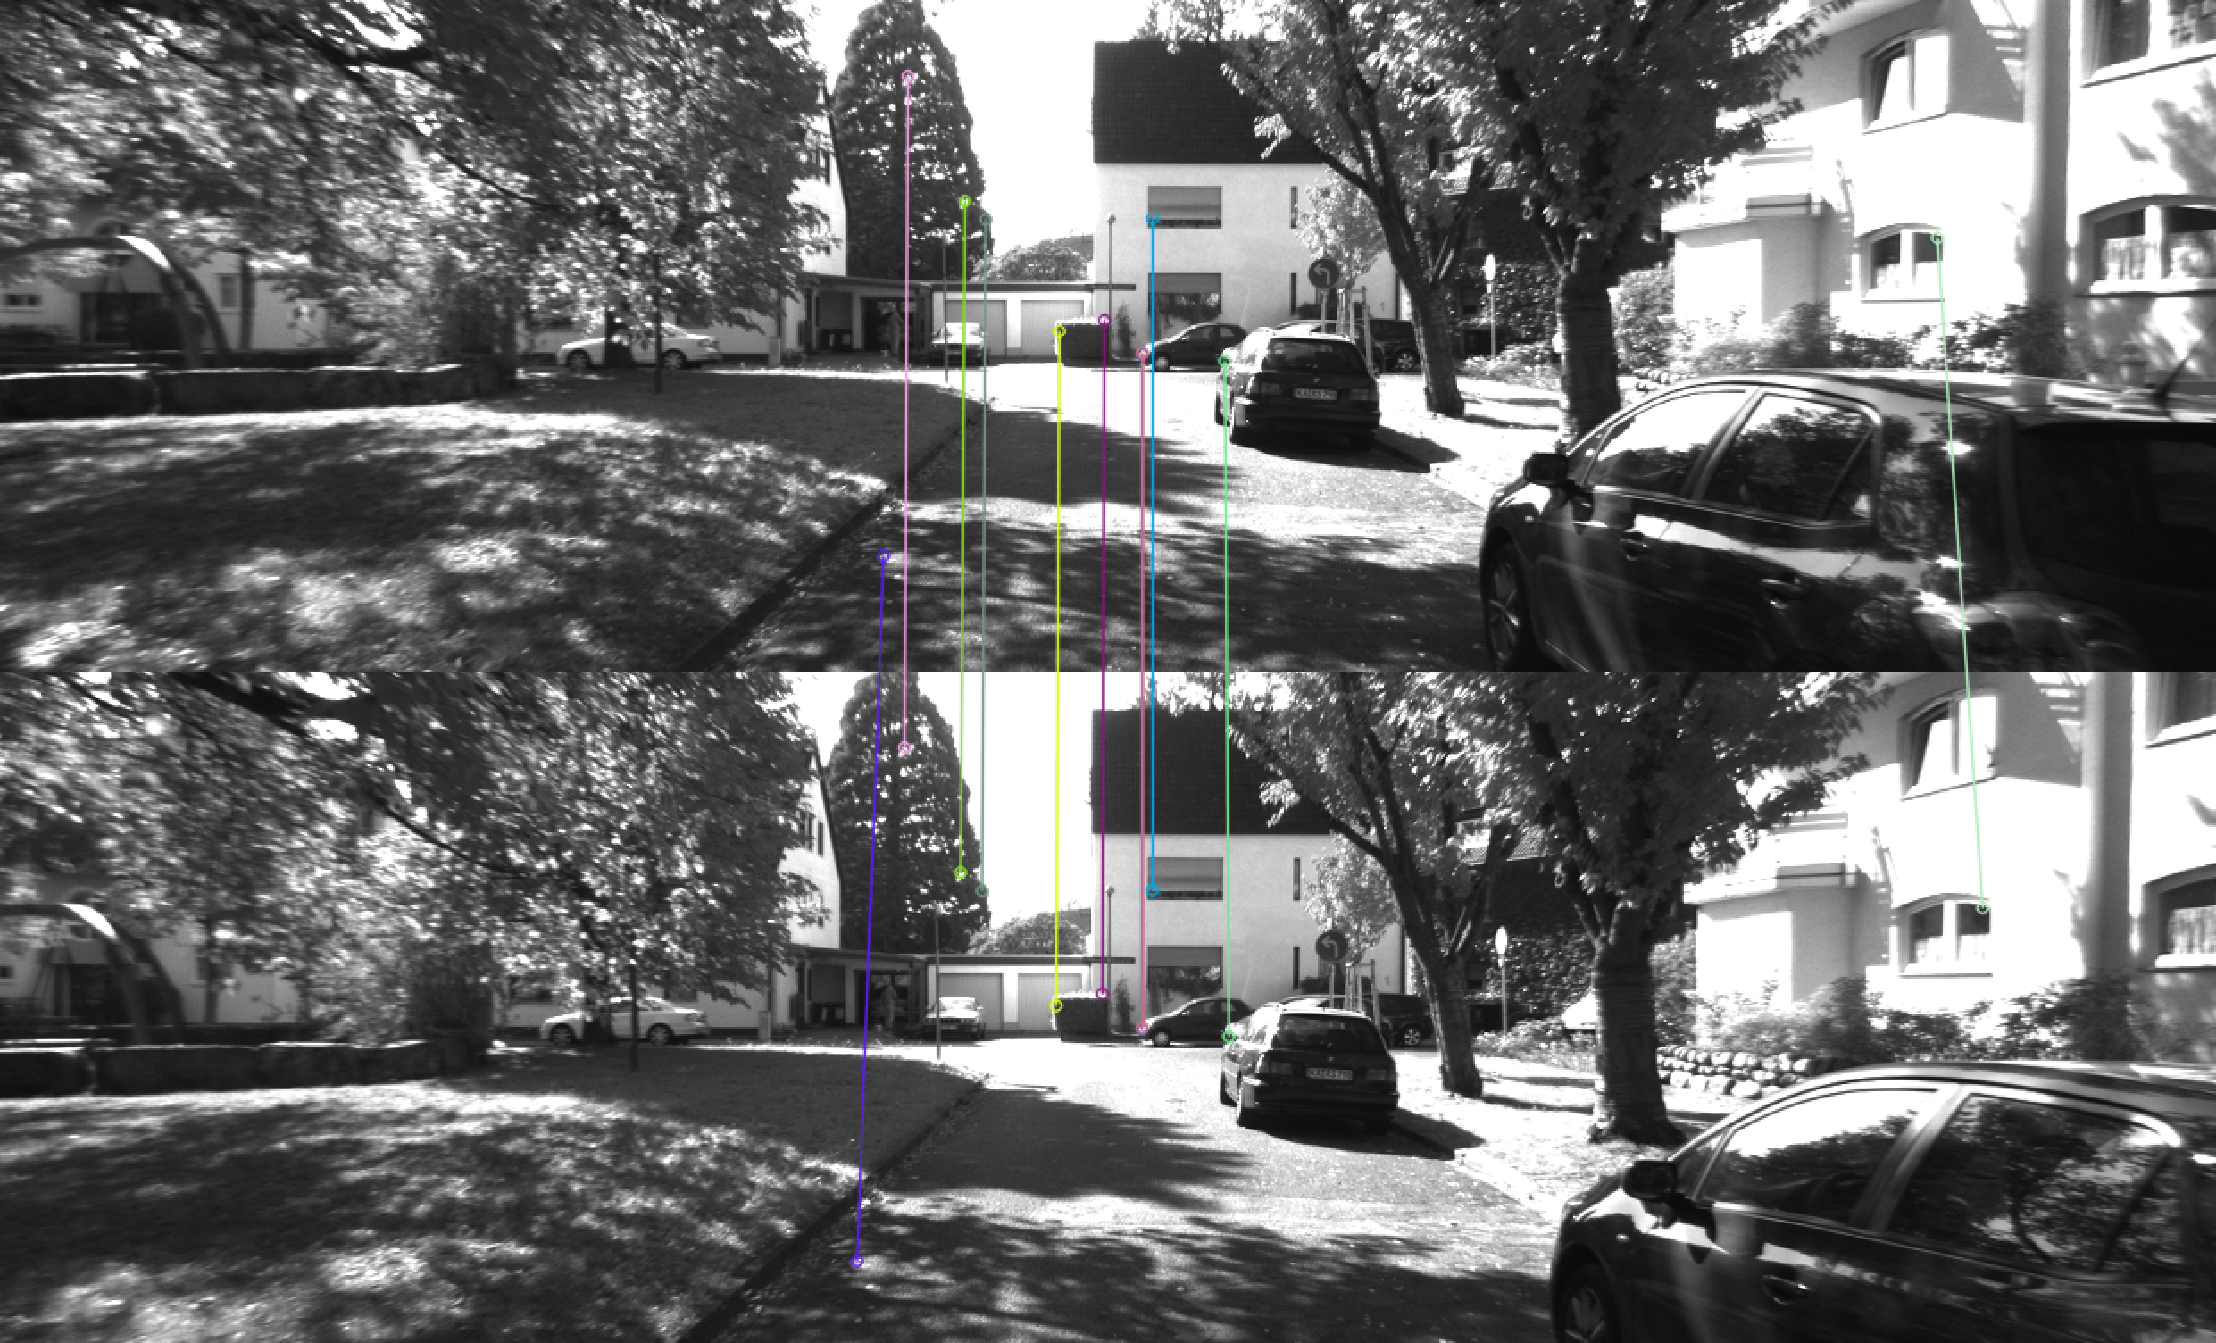
\includegraphics[width=0.9\linewidth]{vo1/feature-matching}
    \caption{两帧图像间的特征匹配。}
    \label{fig:feature-matching}
\end{figure}

不过,让我们先来看正确匹配的情况,等做完实验再回头去讨论误匹配问题。考虑两个时刻的图像。如果在图像$I_{t}$中提取到特征点$ x_{t}^{m}, m=1,2,...,M$,在图像$I_{t+1}$中提取到特征点$x_{t+1}^{n}, n=1,2,...,N$,如何寻找这两个集合元素的对应关系呢?最简单的特征匹配方法就是\textbf{暴力匹配(Brute-Force Matcher)}。即对每一个特征点$x_{t}^{m}$与所有的$x_{t+1}^{n}$测量描述子的距离,然后排序,取最近的一个作为匹配点。描述子距离表示了两个特征之间的\textbf{相似程度},不过在实际运用中还可以取不同的距离度量范数。对于浮点类型的描述子,使用欧氏距离进行度量即可。而对于二进制的描述子(比如BRIEF这样的),我们往往使用汉明距离(Hamming distance)作为度量——两个二进制串之间的汉明距离,指的是其\textbf{不同位数的个数}。

然而,当特征点数量很大时,暴力匹配法的运算量将变得很大,特别是当想要匹配某个帧和一张地图的时候。这不符合我们在SLAM中的实时性需求。此时\textbf{快速近似最近邻(FLANN)}算法更加适合于匹配点数量极多的情况。由于这些匹配算法理论已经成熟,而且实现上也已集成到OpenCV,所以这里就不再描述它的技术细节了。感兴趣的读者可以参考阅读文献\cite{Muja2009}。

\section{实践:特征提取和匹配}
\begin{figure}[!htp]
	\centering
	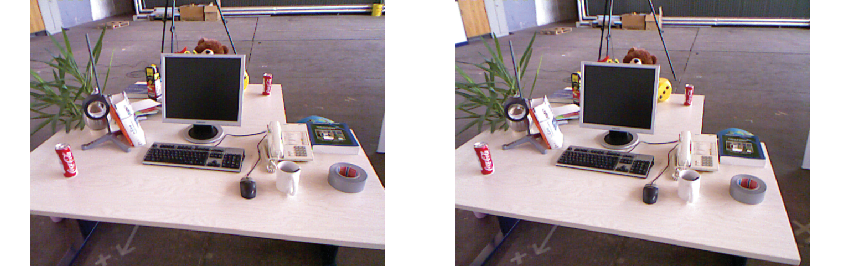
\includegraphics[width=0.9\linewidth]{vo1/exp1-images.pdf}
	\caption{实验使用的两帧图像。}
	\label{fig:exp1-images}
\end{figure}

OpenCV已经集成了多数主流的图像特征,我们可以很方便地进行调用。下面我们来完成两个实验:第一个实验中,我们演示使用OpenCV进行ORB的特征匹配;第二个实验中,我们演示如何根据前面介绍的原理,手写一个简单的ORB特征。通过手写的过程,读者可以更加清楚地理解ORB的计算过程,并类推到其他特征上去。

\subsection{OpenCV的ORB特征}
首先我们调用OpenCV来提取和匹配ORB。我为此实验准备了两张图像,位于slambook2/ch7/下的1.png和2.png,如\autoref{fig:exp1-images}~所示。它们是来自公开数据集\cite{Sturm2012}中的两张图像,我们看到相机发生了微小的运动。本节程序演示如何提取ORB特征并进行匹配。下一小节中,我们将演示如何用匹配结果来估计相机运动。

下面程序演示了ORB的使用方法:
\begin{lstlisting}[language=c++,caption=slambook2/ch7/orb_cv.cpp]
#include <iostream>
#include <opencv2/core/core.hpp>
#include <opencv2/features2d/features2d.hpp>
#include <opencv2/highgui/highgui.hpp>
#include <chrono>

using namespace std;
using namespace cv;

int main(int argc, char **argv) {
    if (argc != 3) {
        cout << "usage: feature_extraction img1 img2" << endl;
        return 1;
    }
    //-- 读取图像
    Mat img_1 = imread(argv[1], CV_LOAD_IMAGE_COLOR);
    Mat img_2 = imread(argv[2], CV_LOAD_IMAGE_COLOR);
    assert(img_1.data != nullptr && img_2.data != nullptr);
    
    //-- 初始化
    std::vector<KeyPoint> keypoints_1, keypoints_2;
    Mat descriptors_1, descriptors_2;
    Ptr<FeatureDetector> detector = ORB::create();
    Ptr<DescriptorExtractor> descriptor = ORB::create();
    Ptr<DescriptorMatcher> matcher = DescriptorMatcher::create("BruteForce-Hamming");
    
    //-- 第一步:检测 Oriented FAST 角点位置
    chrono::steady_clock::time_point t1 = chrono::steady_clock::now();
    detector->detect(img_1, keypoints_1);
    detector->detect(img_2, keypoints_2);
    
    //-- 第二步:根据角点位置计算 BRIEF 描述子
    descriptor->compute(img_1, keypoints_1, descriptors_1);
    descriptor->compute(img_2, keypoints_2, descriptors_2);
    chrono::steady_clock::time_point t2 = chrono::steady_clock::now();
    chrono::duration<double> time_used = chrono::duration_cast<chrono::duration<double>>(t2 - t1);
    cout << "extract ORB cost = " << time_used.count() << " seconds. " << endl;
    
    Mat outimg1;
    drawKeypoints(img_1, keypoints_1, outimg1, Scalar::all(-1), DrawMatchesFlags::DEFAULT);
    imshow("ORB features", outimg1);
    
    //-- 第三步:对两幅图像中的BRIEF描述子进行匹配,使用 Hamming 距离
    vector<DMatch> matches;
    t1 = chrono::steady_clock::now();
    matcher->match(descriptors_1, descriptors_2, matches);
    t2 = chrono::steady_clock::now();
    time_used = chrono::duration_cast<chrono::duration<double>>(t2 - t1);
    cout << "match ORB cost = " << time_used.count() << " seconds. " << endl;
    
    //-- 第四步:匹配点对筛选
    // 计算最小距离和最大距离
    auto min_max = minmax_element(matches.begin(), matches.end(),
        [](const DMatch &m1, const DMatch &m2) { return m1.distance < m2.distance; });
    double min_dist = min_max.first->distance;
    double max_dist = min_max.second->distance;
    
    printf("-- Max dist : %f \n", max_dist);
    printf("-- Min dist : %f \n", min_dist);
    
    //当描述子之间的距离大于两倍的最小距离时,即认为匹配有误.但有时候最小距离会非常小,设置一个经验值30作为下限.
    std::vector<DMatch> good_matches;
    for (int i = 0; i < descriptors_1.rows; i++) {
        if (matches[i].distance <= max(2 * min_dist, 30.0)) {
            good_matches.push_back(matches[i]);
        }
    }
    
    //-- 第五步:绘制匹配结果
    Mat img_match;
    Mat img_goodmatch;
    drawMatches(img_1, keypoints_1, img_2, keypoints_2, matches, img_match);
    drawMatches(img_1, keypoints_1, img_2, keypoints_2, good_matches, img_goodmatch);
    imshow("all matches", img_match);
    imshow("good matches", img_goodmatch);
    waitKey(0);
    
    return 0;
}
\end{lstlisting}

运行此程序(需要输入两个图像位置),将输出运行结果:
\begin{lstlisting}[language=sh,caption=终端输入:]
% build/orb_cv 1.png 2.png
extract ORB cost = 0.0229183 seconds. 
match ORB cost = 0.000751868 seconds.
-- Max dist : 95.000000 
-- Min dist : 4.000000 
\end{lstlisting}

\autoref{fig:exp1-results}~显示了例程的运行结果。我们看到未筛选的匹配中带有大量的误匹配。经过一次筛选之后,匹配数量减少了许多,但大多数匹配都是正确的。这里,筛选的依据是\textbf{汉明距离小于最小距离的两倍},这是一种工程上的经验方法,不一定有理论依据。不过,尽管在示例图像中能够筛选出正确的匹配,但我们仍然不能保证在所有其他图像中得到的匹配都是正确的。因此,在后面的运动估计中,还需要使用去除误匹配的算法。在我的机器上,ORB提取花费了22.9毫秒(两张图像),匹配花费了0.75毫秒,可见大部分计算量花在了特征提取上。

\begin{figure}[!htp]
	\centering
	\includegraphics[width=1.0\linewidth]{vo1/exp1-result}
	\caption{特征提取与匹配结果。}
	\label{fig:exp1-results} 
\end{figure}

\subsection{手写ORB特征}
下面我们演示手写ORB特征的方法。这部分代码比较多,书上只展示核心部分的代码,其余的周边代码请读者从代码库中获取。
\begin{lstlisting}[language=c++,caption=slambook2/ch7/orb_self.cpp(片段)]
typedef vector<uint32_t> DescType;
// ... 省略图片读取部分代码和测试代码
// compute the descriptor
void ComputeORB(const cv::Mat &img, vector<cv::KeyPoint> &keypoints, vector<DescType> &descriptors) {
    const int half_patch_size = 8;
    const int half_boundary = 16;
    int bad_points = 0;
    for (auto &kp: keypoints) {
        if (kp.pt.x < half_boundary || kp.pt.y < half_boundary ||
        kp.pt.x >= img.cols - half_boundary || kp.pt.y >= img.rows - half_boundary) {
            // outside
            bad_points++;
            descriptors.push_back({});
            continue;
        }
    
        float m01 = 0, m10 = 0;
        for (int dx = -half_patch_size; dx < half_patch_size; ++dx) {
            for (int dy = -half_patch_size; dy < half_patch_size; ++dy) {
                uchar pixel = img.at<uchar>(kp.pt.y + dy, kp.pt.x + dx);
                m01 += dx * pixel;
                m10 += dy * pixel;
            }
        }
    
        // angle should be arc tan(m01/m10);
        float m_sqrt = sqrt(m01 * m01 + m10 * m10);
        float sin_theta = m01 / m_sqrt;
        float cos_theta = m10 / m_sqrt;
        
        // compute the angle of this point
        DescType desc(8, 0);
        for (int i = 0; i < 8; i++) {
            uint32_t d = 0;
            for (int k = 0; k < 32; k++) {
                int idx_pq = i * 8 + k;
                cv::Point2f p(ORB_pattern[idx_pq * 4], ORB_pattern[idx_pq * 4 + 1]);
                cv::Point2f q(ORB_pattern[idx_pq * 4 + 2], ORB_pattern[idx_pq * 4 + 3]);
        
                // rotate with theta
                cv::Point2f pp = cv::Point2f(cos_theta * p.x - sin_theta * p.y, sin_theta * p.x + cos_theta * p.y) + kp.pt;
                cv::Point2f qq = cv::Point2f(cos_theta * q.x - sin_theta * q.y, sin_theta * q.x + cos_theta * q.y) + kp.pt;
                if (img.at<uchar>(pp.y, pp.x) < img.at<uchar>(qq.y, qq.x)) {
                    d |= 1 << k;
                }
            }
            desc[i] = d;
        }
        descriptors.push_back(desc);
    }
    
    cout << "bad/total: " << bad_points << "/" << keypoints.size() << endl;
}

// brute-force matching
void BfMatch(
    const vector<DescType> &desc1, const vector<DescType> &desc2, vector<cv::DMatch> &matches) {
    const int d_max = 40;
    
    for (size_t i1 = 0; i1 < desc1.size(); ++i1) {
        if (desc1[i1].empty()) continue;
        cv::DMatch m{i1, 0, 256};
        for (size_t i2 = 0; i2 < desc2.size(); ++i2) {
            if (desc2[i2].empty()) continue;
            int distance = 0;
            for (int k = 0; k < 8; k++) {
                distance += _mm_popcnt_u32(desc1[i1][k] ^desc2[i2][k]);
            }
            if (distance < d_max && distance < m.distance) {
                m.distance = distance;
                m.trainIdx = i2;
            }
        }
        if (m.distance < d_max) {
            matches.push_back(m);
        }
    }
}
\end{lstlisting}
这个演示中我们只展示ORB的计算代码和匹配代码。在计算中,我们用256位的二进制描述,即对应到8个32位的unsigned int数据,用typedef将它表示成DescType。然后,我们根据前面介绍的原理计算FAST特征点的角度,再使用该角度计算描述子。此代码中通过三角函数的原理回避了复杂的$\arctan$以及$\sin$、$\cos$计算,从而达到加速的效果。在BfMatch函数中,我们还使用了SSE指令集中的\_mm\_popcnt\_u32函数来计算一个unsigned int变量中1的个数,从而达到计算汉明距离的效果。该段程序的运行结果如下,匹配结果如\autoref{fig:matches}所示:

\begin{lstlisting}[language=sh,caption=终端输出:]
bad/total: 43/638
bad/total: 8/595
extract ORB cost = 0.00390721 seconds.
match ORB cost = 0.000862984 seconds.
matches: 51
\end{lstlisting}

\begin{figure}[!htp]
    \centering
    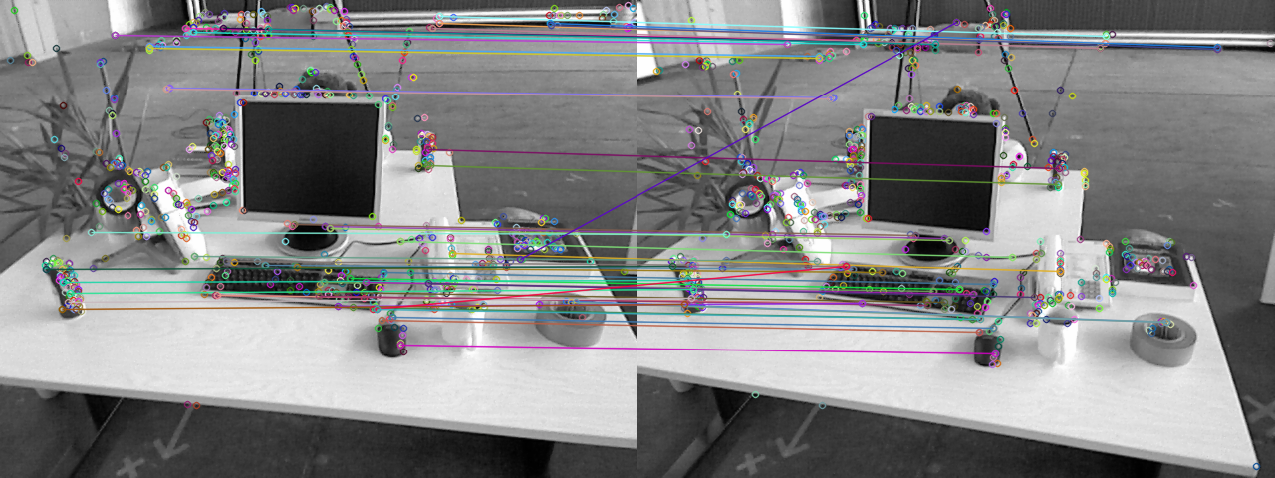
\includegraphics[width=0.8\linewidth]{vo1/matches}
    \caption{匹配结果}
    \label{fig:matches}
\end{figure}

可见,这个程序中,ORB的提取只需要3.9毫秒,匹配只需0.86毫秒。我们通过一些简单的算法修改,对ORB的提取加速了5.8倍。请读者注意,编译这个程序需要你的CPU支持SSE指令集,这应该在绝大多数现代的家用CPU上都已经支持。如果我们能够对提取特征部分进一步并行化处理,算法还可以有加速的空间。

\subsection{计算相机运动}
我们已经有了匹配好的点对,接下来,我们要根据点对来估计相机的运动。这里由于相机的原理不同,情况发生了变化:

\begin{enumerate}
	\item 当相机为单目时,我们只知道2D的像素坐标,因而问题是根据\textbf{两组2D点}估计运动。该问题用\textbf{对极几何}来解决。
	\item 当相机为双目、RGB-D时,或者通过某种方法得到了距离信息,那么问题就是根据\textbf{两组3D点}估计运动。该问题通常用ICP来解决。
	\item 如果一组为3D,一组为2D,即,我们得到了一些3D点和它们在相机的投影位置,也能估计相机的运动。该问题通过\textbf{PnP}求解。
\end{enumerate}

因此,下面几节就来介绍这三种情形下的相机运动估计。我们将从信息最少的2D−2D情形出发,看看它如何求解,求解过程又有哪些麻烦的问题。

\section{2D−2D: 对极几何}
\label{sec:epipolar-geometry}

\subsection{对极约束}

现在,假设我们从两张图像中得到了一对配对好的特征点,如\autoref{fig:doubleview}~所示。如果有若干对这样的匹配点,就可以通过这些二维图像点的对应关系,恢复出在两帧之间摄像机的运动。这里“若干对”具体是多少对呢?我们会在下文介绍。下面先来看看两个图像当中的匹配点有什么几何关系。

\begin{figure}[!htp]
	\centering
	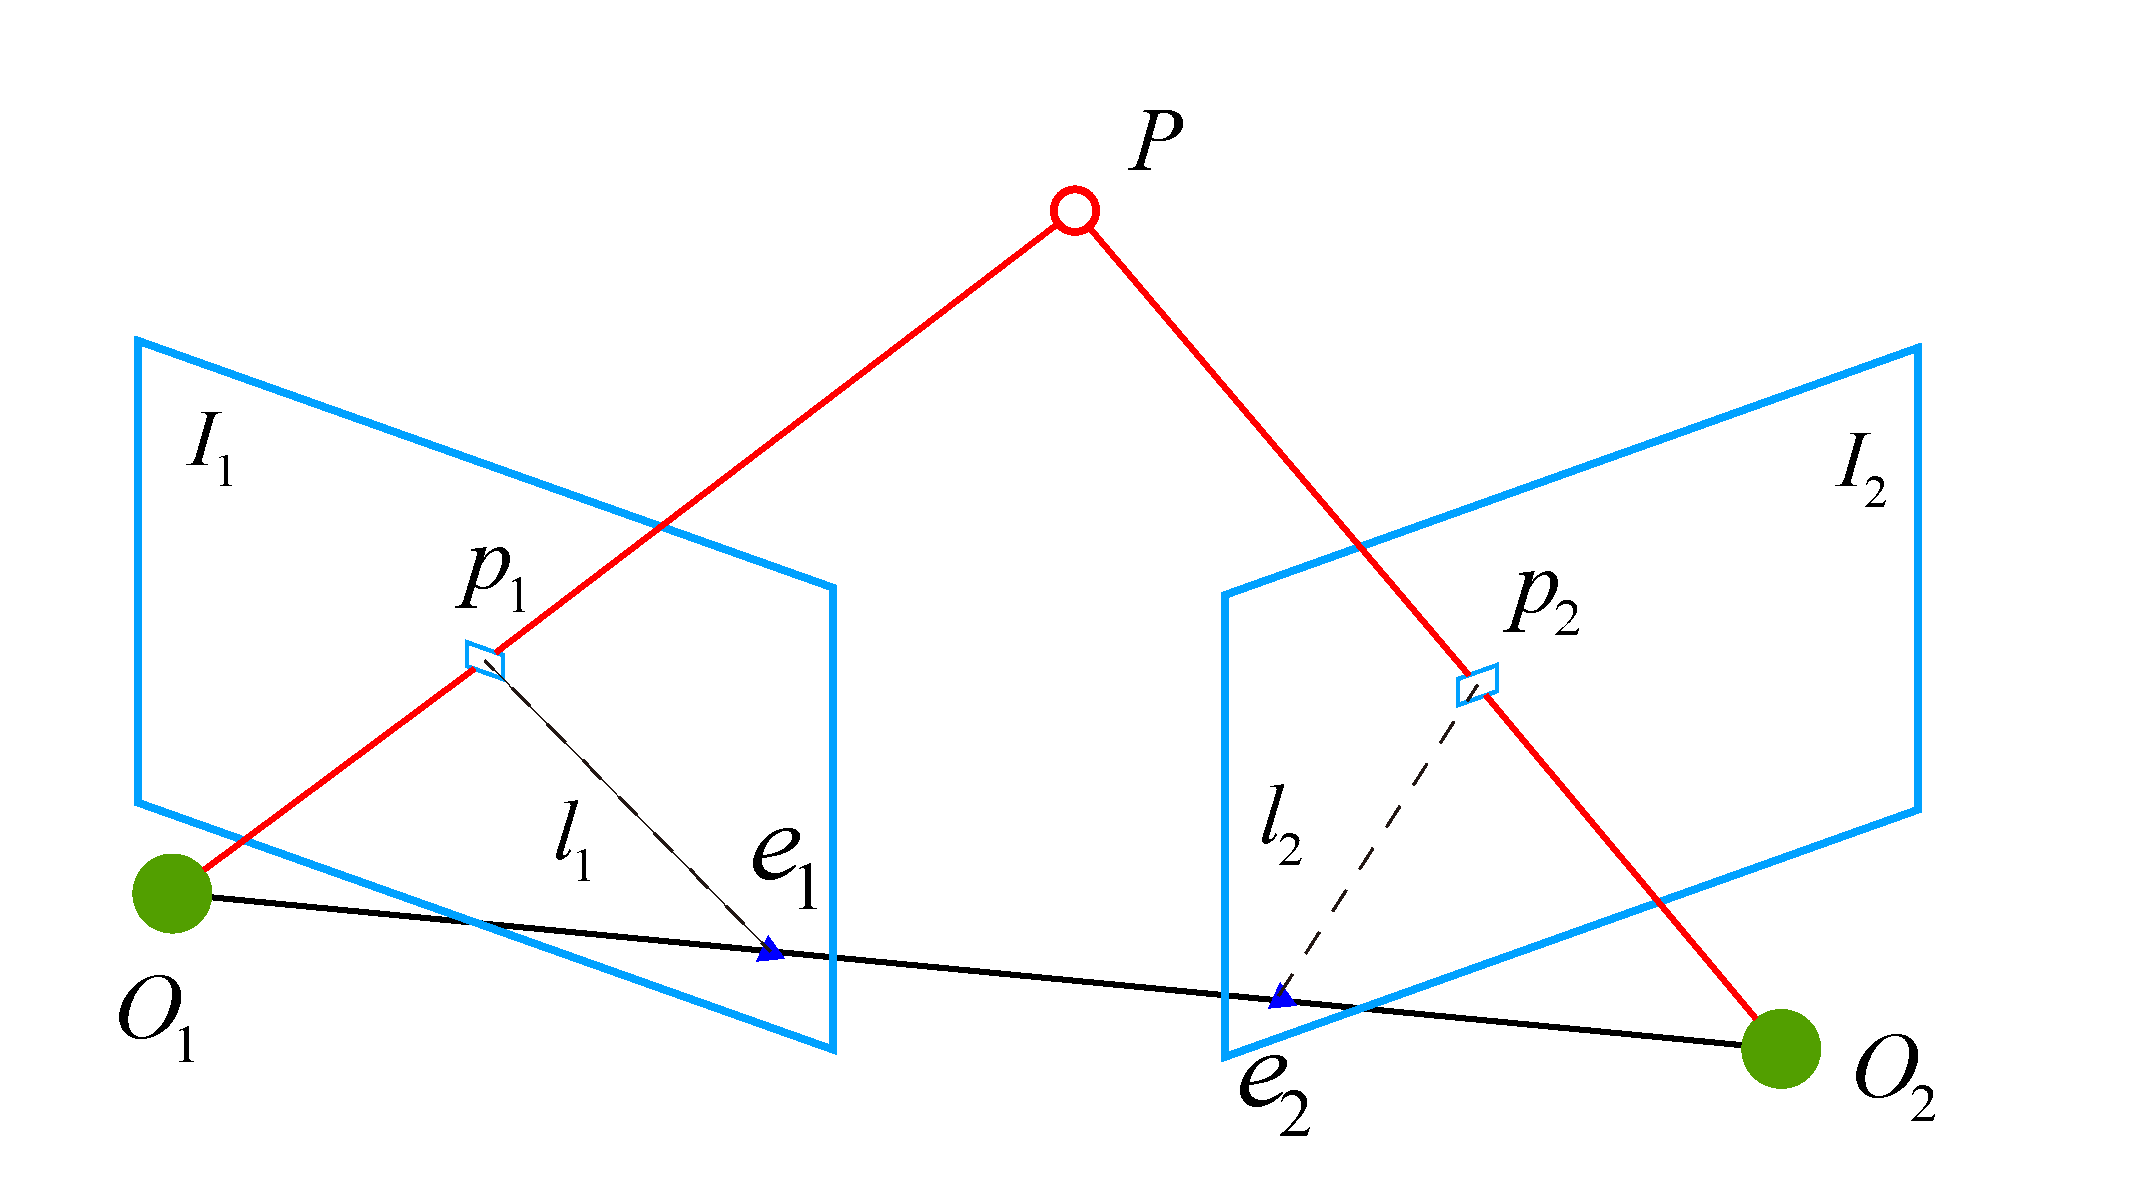
\includegraphics[width=0.6\linewidth]{vo1/fundamental}
	\caption{对极几何约束。}
	\label{fig:doubleview}
\end{figure}

以\autoref{fig:doubleview}~为例,我们希望求取两帧图像$I_{1}, I_{2}$之间的运动,设第一帧到第二帧的运动为$\bm{R}, \bm{t}$。两个相机中心分别为$O_{1}, O_{2}$。现在,考虑$I_{1}$中有一个特征点$p_{1}$,它在$I_{2}$中对应着特征点$p_{2}$。我们知道两者是通过特征匹配得到的。如果匹配正确,说明它们确实是\textbf{同一个空间点在两个成像平面上的投影}。这里需要一些术语来描述它们之间的几何关系。首先,连线$\overrightarrow{O_{1}p_{1}}$和连线$\overrightarrow{O_{2}p_{2}}$在三维空间中会相交于点$P$。这时候点$O_{1},O_{2},P$三个点可以确定一个平面,称为\textbf{极平面(Epipolar plane)}。$O_{1}O_{2}$连线与像平面$I_{1},I_{2}$的交点分别为$e_{1},e_{2}$。$e_{1},e_{2}$称为\textbf{极点(Epipoles)},$O_{1}O_{2}$被称为\textbf{基线(Baseline)}。我们称极平面与两个像平面$I_{1}, I_{2}$之间的相交线$l_{1},l_{2}$为\textbf{极线(Epipolar line)}。

直观讲,从第一帧的角度看,射线$\overrightarrow{O_1 p_1}$是\textbf{某个像素可能出现的空间位置}——因为该射线上的所有点都会投影到同一个像素点。同时,如果不知道$P$的位置,那么当我们在第二幅图像上看时,连线$\overrightarrow{e_2 p_2}$(也就是第二幅图像中的极线)就是$P$可能出现的投影的位置,也就是射线$\overrightarrow{O_1 p_1}$在第二个相机中的投影。现在,由于我们通过特征点匹配确定了$p_2$的像素位置,所以能够推断$P$的空间位置,以及相机的运动。要提醒读者的是,\textbf{这多亏了正确的特征匹配}。如果没有特征匹配,我们就没法确定$p_2$到底在极线的哪个位置了。那时,就必须在极线上搜索以获得正确的匹配,这将在第12讲中提到。

现在,我们从代数角度来看一下这里的几何关系。在第一帧的坐标系下,设$P$的空间位置为
\[
\bm{P}=[X,Y,Z]^\mathrm{T}.
\]
根据第5讲介绍的针孔相机模型,我们知道两个像素点$\bm{p}_1,\bm{p}_2$的像素位置为
\begin{equation}
s_1 {\bm{p}_1} = \bm{KP},\quad s_2 \bm{p}_2 = \bm{K}\left( \bm{RP + t} \right).
\end{equation}

这里$\bm{K}$为相机内参矩阵,$\bm{R}, \bm{t}$为两个坐标系的相机运动。具体来说,这里计算的是$\bm{R}_{21}$和$\bm{t}_{21}$,因为它们把第一个坐标系下的坐标转换到第二个坐标系下。如果我们愿意,也可以把它们写成李代数形式。

有时候,我们会使用齐次坐标表示像素点。在使用齐次坐标时,一个向量将等于它自身乘上任意的非零常数。这通常用于表达一个投影关系。例如$s_1 \bm{p}_1$和$\bm{p}_1$成投影关系,它们在齐次坐标的意义下是相等的。我们称这种相等关系为\textbf{尺度意义下相等}(equal up to a scale),记作:
\begin{equation}
s\bm{p} \simeq \bm{p}.
\end{equation}
那么,上述两个投影关系可写为:
\begin{equation}
 {\bm{p}_1} \simeq \bm{KP},\quad \bm{p}_2 \simeq \bm{K}\left( \bm{RP + t} \right).
\end{equation}

现在,取:
\begin{equation}
{\bm{x}_1} = {\bm{K}^{ - 1}}{\bm{p}_1}, \quad {\bm{x}_2} = {\bm{K}^{ - 1}}{\bm{p}_2}.
\end{equation}

这里的$\bm{x}_1, \bm{x}_2$是两个像素点的归一化平面上的坐标。代入上式,得:
\begin{equation}
{\bm{x}_2} \simeq \bm{R} {\bm{x}_1} + \bm{t}.
\end{equation}

两边同时左乘$\bm{t}^\wedge$。回忆$^\wedge$的定义,这相当于两侧同时与$\bm{t}$做外积:
\begin{equation}
\bm{t}^\wedge \bm{x}_2 \simeq \bm{t}^\wedge \bm{R} \bm{x}_1.
\end{equation}

然后,两侧同时左乘$\bm{x}_2^\mathrm{T}$:
\begin{equation}
\bm{x}_2^\mathrm{T} \bm{t}^\wedge \bm{x}_2 \simeq \bm{x}_2^\mathrm{T} \bm{t}^\wedge \bm{R} \bm{x}_1.
\end{equation}

观察等式左侧,$\bm{t}^\wedge \bm{x}_2$是一个与$\bm{t}$和$\bm{x}_2$都垂直的向量。把它再和$\bm{x}_2$做内积时,将得到0。由于等式左侧严格为零,那么乘以任意非零常数之后也为零,于是我们可以把$\simeq$写成通常的等号。因此,我们就得到了一个简洁的式子:
\begin{equation}
 \bm{x}_2^\mathrm{T} \bm{t}^\wedge \bm{R} \bm{x}_1 = 0.
\end{equation}

重新代入$\bm{p}_1, \bm{p}_2$,有:
\begin{equation}
\bm{p}_2^\mathrm{T} \bm{K}^{-\mathrm{T}} \bm{t}^\wedge \bm{R} \bm{K}^{-1} \bm{p}_1  = 0.
\end{equation}

这两个式子都称为\textbf{对极约束},它以形式简洁著名。它的几何意义是$O_1, P, O_2$三者共面。对极约束中同时包含了平移和旋转。我们把中间部分记作两个矩阵:基础矩阵(Fundamental Matrix)$\bm{F}$和本质矩阵(Essential Matrix)$\bm{E}$,于是可以进一步简化对极约束:
\begin{equation}
\bm{E} = \bm{t}^ \wedge \bm{R}, \quad \bm{F} = \bm{K}^{ -\mathrm{T}} \bm{E} {\bm{K}^{ - 1}}, \quad \bm{x}_2^\mathrm{T} \bm{E} {\bm{x}_1} = \bm{p}_2^\mathrm{T} \bm{F} {\bm{p}_1} = 0.
\end{equation}

对极约束简洁地给出了两个匹配点的空间位置关系。于是,相机位姿估计问题变为以下两步:

\begin{enumerate}
	\item 根据配对点的像素位置求出$\bm{E}$或者$\bm{F}$。
	\item 根据$\bm{E}$或者$\bm{F}$求出$\bm{R}, \bm{t}$。
\end{enumerate}

由于$\bm{E}$和$\bm{F}$只相差了相机内参,而内参在SLAM中通常是已知的\footnote{在SfM研究中则有可能是未知而有待估计的。},所以实践当中往往使用形式更简单的$\bm{E}$。我们以$\bm{E}$为例,介绍上面两个问题如何求解。

\subsection{本质矩阵}
根据定义,本质矩阵$\bm{E} = \bm{t}^\wedge \bm{R}$。它是一个$3\times 3$的矩阵,内有9个未知数。那么,是不是任意一个$3 \times 3$的矩阵都可以被当成本质矩阵呢?从$\bm{E}$的构造方式上看,有以下值得注意的地方:

\begin{itemize}
	\item 本质矩阵是由对极约束定义的。由于对极约束是\textbf{等式为零}的约束,所以对$\bm{E}$乘以任意非零常数后,\textbf{对极约束依然满足}。我们把这件事情称为$\bm{E}$在不同尺度下是等价的。
	\item 根据$\bm{E} = \bm{t}^ \wedge \bm{R}$,可以证明\textsuperscript{\cite{Hartley2003}},本质矩阵$\bm{E}$的奇异值必定是$[\sigma, \sigma, 0]^\mathrm{T}$的形式。这称为\textbf{本质矩阵的内在性质}。
	\item 另一方面,由于平移和旋转各有3个自由度,故$\bm{t}^\wedge \bm{R}$共有6个自由度。但由于尺度等价性,故$\bm{E}$实际上有5个自由度。
\end{itemize}

$\bm{E}$具有5个自由度的事实,表明我们最少可以用5对点来求解$\bm{E}$。但是,$\bm{E}$的内在性质是一种非线性性质,在估计时会带来麻烦,因此,也可以只考虑它的\textbf{尺度等价性},使用8对点来估计$\bm{E}$——这就是经典的\textbf{八点法(Eight-point-algorithm)}\textsuperscript{\cite{Hartley1997, Longuet-Higgins1987}}。八点法只利用了$\bm{E}$的线性性质,因此可以在线性代数框架下求解。下面我们来看八点法是如何工作的。

考虑一对匹配点,它们的归一化坐标为$\bm{x}_{1}=[u_{1},v_{1},1]^\mathrm{T}$, $\bm{x}_{2}=[u_{2},v_{2},1]^{\mathrm{T}}$。根据对极约束,有:
\begin{equation}
\begin{pmatrix} 
u_{2},v_{2},1
\end{pmatrix}
\begin{pmatrix}
 e_{1} & e_{2} & e_{3}\\ 
 e_{4} & e_{5} & e_{6}\\ 
 e_{7} & e_{8} & e_{9} 
\end{pmatrix}
\begin{pmatrix} 
u_{1}\\v_{1}\\1
\end{pmatrix}
=0.
\end{equation}

我们把矩阵$\bm{E}$展开,写成向量的形式:
\[
\bm{e}= [e_{1},e_{2},e_{3},e_{4},e_{5},e_{6},e_{7},e_{8},e_{9}]^{\mathrm{T}},
\]
那么对极约束可以写成与$\bm{e}$有关的线性形式:
\begin{equation}
[u_{2}u_{1},u_{2}v_{1},u_{2},v_{2}u_{1},v_{2}v_{1},v_{2},u_{1},v_{1},1] \cdot  \bm{e}=0.
\end{equation}

同理,对于其他点对也有相同的表示。我们把所有点都放到一个方程中,变成线性方程组($u^i, v^i$表示第$i$个特征点,依此类推):
\begin{equation}
\label{Eq:eight-point}
\begin{pmatrix}
u_{2}^{1}u_{1}^{1}& u_{2}^{1}v_{1}^{1}& u_{2}^{1}& v_{2}^{1}u_{1}^{1}& v_{2}^{1}v_{1}^{1}& v_{2}^{1} &u_{1}^{1} &v_{1}^{1}&1\\
u_{2}^{2}u_{1}^{2}& u_{2}^{2}v_{1}^{2}& u_{2}^{2}& v_{2}^{2}u_{1}^{2}& v_{2}^{2}v_{1}^{2}& v_{2}^{2} &u_{1}^{2} &v_{1}^{2}&1\\
\vdots & \vdots & \vdots & \vdots & \vdots & \vdots & \vdots & \vdots \\
u_{2}^{8}u_{1}^{8}& u_{2}^{8}v_{1}^{8}& u_{2}^{8}& v_{2}^{8}u_{1}^{8}& v_{2}^{8}v_{1}^{8}& v_{2}^{8} &u_{1}^{8}&v_{1}^{8}&1\\
\end{pmatrix}
\begin{pmatrix}
e_{1}\\ e_{2}\\ e_{3}\\  e_{4}\\ e_{5}\\ e_{6}\\ e_{7}\\ e_{8}\\ e_{9}  
\end{pmatrix}
=0.
\end{equation}

这8个方程构成了一个线性方程组。它的系数矩阵由特征点位置构成,大小为$8 \times 9$。$\bm{e}$位于该矩阵的零空间中。如果系数矩阵是满秩的(即秩为8),那么它的零空间维数为1,也就是$\bm{e}$构成一条线。这与$\bm{e}$的尺度等价性是一致的。如果8对匹配点组成的矩阵满足秩为8的条件,那么$\bm{E}$的各元素就可由上述方程解得。

接下来的问题是如何根据已经估得的本质矩阵$\bm{E}$,恢复出相机的运动$\bm{R}, \bm{t}$。这个过程是由奇异值分解(SVD)得到的。设$\bm{E}$的SVD分解为
\begin{equation}
\bm{E} = \bm{U} \bm{\Sigma} \bm{V}^\mathrm{T},
\end{equation}
其中$\bm{U}, \bm{V}$为正交阵,$\bm{\Sigma}$为奇异值矩阵。根据$\bm{E}$的内在性质,我们知道$\bm{\Sigma} = \mathrm{diag}( \sigma, \sigma, 0 )$。在SVD分解中,对于任意一个$\bm{E}$,存在两个可能的$\bm{t}, \bm{R}$与它对应:
\begin{equation}
\begin{array}{l}
\bm{t}_1^ \wedge  = \bm{U}{\bm{R}_Z}(\frac{\pi }{2}) \bm{\Sigma} {\bm{U}^\mathrm{T}}, \quad {\bm{R}_1} = \bm{U} \bm{R}_Z^\mathrm{T}(\frac{\pi }{2}){ \bm{V}^\mathrm{T}}\\
\bm{t}_2^ \wedge  = \bm{U}{\bm{R}_Z}( - \frac{\pi }{2})\bm{\Sigma} {\bm{U}^\mathrm{T}}, \quad  {\bm{R}_2} = \bm{U} \bm{R}_Z^\mathrm{T}( - \frac{\pi }{2}){\bm{V}^\mathrm{T}}.
\end{array}
\end{equation}

其中$\bm{R}_Z\left(\frac{\pi }{2}\right)$表示沿$Z$轴旋转$90^\circ$得到的旋转矩阵。同时,由于$-\bm{E}$和$\bm{E}$等价,所以对任意一个$\bm{t}$取负号,也会得到同样的结果。因此,从$\bm{E}$分解到$\bm{t}, \bm{R}$时,一共存在\textbf{4个}可能的解。

\autoref{fig:epipolar-solution}~形象地展示了分解本质矩阵得到的4个解。我们已知空间点在相机(蓝色线)上的投影(红色点),想要求解相机的运动。在保持红色点不变的情况下,可以画出4种可能的情况。不过幸运的是,只有第一种解中$P$在两个相机中都具有正的深度。因此,只要把任意一点代入4种解中,检测该点在两个相机下的深度,就可以确定哪个解是正确的了。

\begin{figure}[!htp]
	\centering
	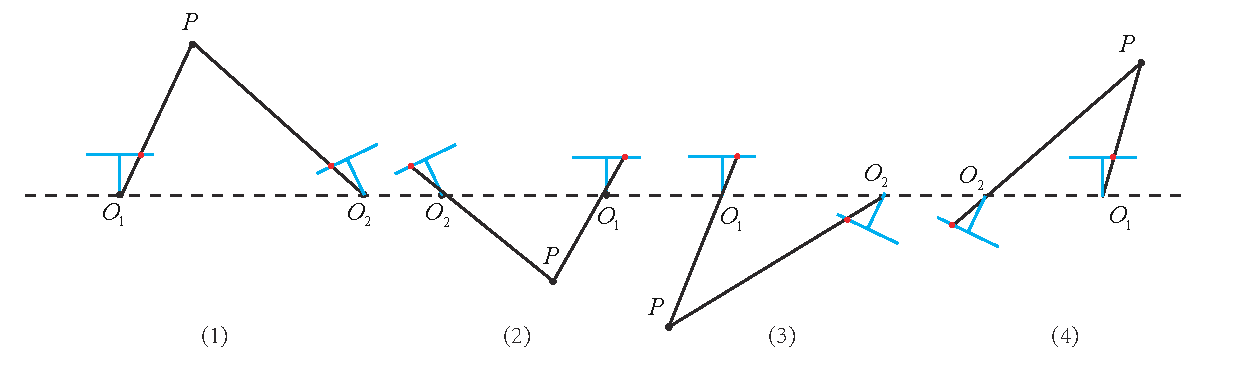
\includegraphics[width=1.0\linewidth]{vo1/epipolar-solution}
	\caption{分解本质矩阵得到的4个解。在保持投影点(红色点)不变的情况下,两个相机及空间点一共有4种可能的情况。}
	\label{fig:epipolar-solution}
\end{figure}

如果利用$\bm{E}$的内在性质,那么它只有5个自由度。所以最少可以通过5对点来求解相机运动\textsuperscript{\cite{Li2006, Nister2004a}}。然而这种做法形式复杂,从工程实现角度考虑,由于平时通常会有几十对乃至上百对的匹配点,从8对减至5对意义并不明显。为保持简单,我们这里就只介绍基本的八点法。

剩下的问题还有一个:根据线性方程解出的$\bm{E}$,可能不满足$\bm{E}$的内在性质——它的奇异值不一定为${\sigma}, {\sigma}, 0$的形式。这时,我们会刻意地把$\bm{\Sigma}$矩阵调整成上面的样子。通常的做法是,对八点法求得的$\bm{E}$进行SVD分解后,会得到奇异值矩阵$\bm{\Sigma} =  \mathrm{diag} ( \sigma_1, \sigma_2, \sigma_3)$,不妨设$\sigma_1 \geqslant \sigma_2 \geqslant \sigma_3$。取:
\begin{equation}
\bm{E} = \bm{U} \mathrm{diag} (\frac{\sigma_1+\sigma_2}{2}, \frac{\sigma_1+\sigma_2}{2}, 0) \bm{V}^\mathrm{T}.
\end{equation}
这相当于是把求出来的矩阵投影到了$\bm{E}$所在的流形上。当然,更简单的做法是将奇异值矩阵取成$\mathrm{diag} (1,1,0)$,因为$\bm{E}$具有尺度等价性,所以这样做也是合理的。

\subsection{单应矩阵}
除了基本矩阵和本质矩阵,二视图几何中还存在另一种常见的矩阵:单应矩阵(Homography)$\bm{H}$,它描述了两个平面之间的映射关系。若场景中的特征点都落在同一平面上(比如墙、地面等),则可以通过单应性来进行运动估计。这种情况在无人机携带的俯视相机或扫地机携带的顶视相机中比较常见。由于之前没有提到过单应,因此这里稍微介绍一下。

单应矩阵通常描述处于共同平面上的一些点在两张图像之间的变换关系。考虑在图像$I_{1}$和$I_{2}$有一对匹配好的特征点$p_{1}$和$p_{2}$。这些特征点落在平面$P$上,设这个平面满足方程:
\begin{equation}
\bm{n}^\mathrm{T} \bm{P} + d = 0.
\end{equation}
稍加整理,得:
\begin{equation}
- \frac{\bm{n}^\mathrm{T} \bm{P} }{d} = 1.
\end{equation}

然后,回顾本节开头的式(7.1),得:
\begin{align*}
\bm{p}_2 &\simeq \bm{K} ( \bm{R} \bm{P} + \bm{t} ) \\ 
&\simeq \bm{K} \left( \bm{R} \bm{P} + \bm{t} \cdot (- \frac{\bm{n}^\mathrm{T} \bm{P} }{d}) \right) \\
&\simeq \bm{K} \left( \bm{R} - \frac{\bm{t} \bm{n}^\mathrm{T} }{d} \right) \bm{P} \\ 
&\simeq \bm{K} \left( \bm{R} - \frac{\bm{t} \bm{n}^\mathrm{T} }{d} \right) \bm{K}^{-1} \bm{p}_1.
\end{align*}

于是,我们得到了一个直接描述图像坐标$\bm{p}_1$和$\bm{p}_2$之间的变换,把中间这部分记为$\bm{H}$,于是:
\begin{equation}
\bm{p}_2 \simeq \bm{H} \bm{p}_1.
\end{equation}

它的定义与旋转、平移及平面的参数有关。与基础矩阵$\bm{F}$类似,单应矩阵$\bm{H}$也是一个$3 \times 3$的矩阵,求解时的思路也和$\bm{F}$类似,同样可以先根据匹配点计算$\bm{H}$,然后将它分解以计算旋转和平移。把上式展开,得:
\begin{equation}
\begin{pmatrix} 
u_{2}\\v_{2}\\1
\end{pmatrix}
\simeq
\begin{pmatrix}
 h_{1} & h_{2} & h_{3}\\ 
 h_{4} & h_{5} & h_{6}\\ 
 h_{7} & h_{8} & h_{9} 
\end{pmatrix}
\begin{pmatrix} 
u_{1}\\v_{1}\\1
\end{pmatrix}.
\end{equation}

请注意,这里的等号依然是$\simeq$而不是普通的等号,所以$\bm{H}$矩阵也可以乘以任意非零常数。我们在实际处理中可以令$h_9 = 1$(在它取非零值时)。然后根据第3行,去掉这个非零因子,于是有:
\[
\begin{aligned}
u_{2}&=\frac{h_{1}u_{1}+h_{2}v_{1}+h_{3}}{h_{7}u_{1}+h_{8}v_{1}+h_{9}}\\
v_{2}&=\frac{h_{4}u_{1}+h_{5}v_{1}+h_{6}}{h_{7}u_{1}+h_{8}v_{1}+h_{9}}.
\end{aligned}
\]
整理得:
\[
\begin{gathered}
h_{1}u_{1}+h_{2}v_{1}+h_{3}-h_{7}u_{1}u_{2}-h_{8}v_{1}u_{2}=u_{2}\\
h_{4}u_{1}+h_{5}v_{1}+h_{6}-h_{7}u_{1}v_{2}-h_{8}v_{1}v_{2}=v_{2}.
\end{gathered}
\]

这样一组匹配点对就可以构造出两项约束(事实上有三个约束,但是因为线性相关,只取前两个),于是自由度为8的单应矩阵可以通过4对匹配特征点算出(在非退化的情况下,即这些特征点不能有三点共线的情况),即求解以下的线性方程组(当$h_9 = 0$时,右侧为零):
\begin{equation}
\begin{pmatrix}
u_{1}^{1}& v_{1}^{1}& 1 & 0 & 0 & 0 & -u_{1}^{1}u_{2}^{1} & -v_{1}^{1}u_{2}^{1}\\
0 & 0 & 0& u_{1}^{1}& v_{1}^{1}& 1 &  -u_{1}^{1}v_{2}^{1} & -v_{1}^{1}v_{2}^{1}\\
u_{1}^{2}& v_{1}^{2}& 1 & 0 & 0 & 0 & -u_{1}^{2}u_{2}^{2} & -v_{1}^{2}u_{2}^{2}\\
0 & 0 & 0& u_{1}^{2}& v_{1}^{2}& 1 &  -u_{1}^{2}v_{2}^{2} & -v_{1}^{2}v_{2}^{2}\\
u_{1}^{3}& v_{1}^{3}& 1 & 0 & 0 & 0 & -u_{1}^{3}u_{2}^{3} & -v_{1}^{3}u_{2}^{3}\\
0 & 0 & 0& u_{1}^{3}& v_{1}^{3}& 1 &  -u_{1}^{3}v_{2}^{3} & -v_{1}^{3}v_{2}^{3}\\
u_{1}^{4}& v_{1}^{4}& 1 & 0 & 0 & 0 & -u_{1}^{4}u_{2}^{4} & -v_{1}^{4}u_{2}^{4}\\
0 & 0 & 0& u_{1}^{4}& v_{1}^{4}& 1 &  -u_{1}^{4}v_{2}^{4} & -v_{1}^{4}v_{2}^{4}
\end{pmatrix}
\begin{pmatrix}
 h_{1}\\h_{2}\\h_{3}\\ h_{4}\\h_{5}\\h_{6}\\ h_{7}\\h_{8}\\  
\end{pmatrix}
=
\begin{pmatrix}
u_{2}^{1}\\ v_{2}^{1}\\ u_{2}^{2}\\ v_{2}^{2}\\u_{2}^{3}\\ v_{2}^{3}\\u_{2}^{4}\\ v_{2}^{4}
\end{pmatrix}.
\end{equation}

这种做法把$\bm{H}$矩阵看成了向量,通过解该向量的线性方程来恢复$\bm{H}$,又称直接线性变换法(Direct Linear Transform)。与本质矩阵相似,求出单应矩阵以后需要对其进行分解,才可以得到相应的旋转矩阵$\bm{R}$和平移向量$\bm{t}$。分解的方法包括数值法\textsuperscript{\cite{faugeras1988motion, Zhang1996}}与解析法\textsuperscript{\cite{malis2007deeper}}。与本质矩阵的分解类似,单应矩阵的分解同样会返回4组旋转矩阵与平移向量,并且同时可以计算出它们分别对应的场景点所在平面的法向量。如果已知成像的地图点的深度全为正值(即在相机前方),则又可以排除两组解。最后仅剩两组解,这时需要通过更多的先验信息进行判断。通常我们可以通过假设已知场景平面的法向量来解决,如场景平面与相机平面平行,那么法向量$\bm{n}$的理论值为$\bm{1}^\mathrm{T}$。

单应性在SLAM中具有重要意义。当特征点共面或者相机发生纯旋转时,基础矩阵的自由度下降,这就出现了所谓的退化(degenerate)。现实中的数据总包含一些噪声,这时候如果继续使用八点法求解基础矩阵,基础矩阵多余出来的自由度将会主要由噪声决定。为了能够避免退化现象造成的影响,通常我们会同时估计基础矩阵$\bm{F}$和单应矩阵$\bm{H}$,选择重投影误差比较小的那个作为最终的运动估计矩阵。

\section{实践:对极约束求解相机运动}
下面,我们来练习一下如何通过本质矩阵求解相机运动。上一节实践部分的程序提供了特征匹配,而这次我们就使用匹配好的特征点来计算$\bm{E}, \bm{F}$和$\bm{H}$,进而分解$\bm{E}$得到$\bm{R}, \bm{t}$。整个程序使用OpenCV提供的算法进行求解。我们把上一节的特征提取封装成函数,以供后面使用。本节只展示位姿估计部分的代码。

\begin{lstlisting}[language=c++,caption=slambook2/ch7/pose_estimation_2d2d.cpp (片段)]
void pose_estimation_2d2d(std::vector<KeyPoint> keypoints_1,
    std::vector<KeyPoint> keypoints_2,
    std::vector<DMatch> matches,
    Mat &R, Mat &t) {
    // 相机内参,TUM Freiburg2
    Mat K = (Mat_<double>(3, 3) << 520.9, 0, 325.1, 0, 521.0, 249.7, 0, 0, 1);
    
    //-- 把匹配点转换为vector<Point2f>的形式
    vector<Point2f> points1;
    vector<Point2f> points2;
    
    for (int i = 0; i < (int) matches.size(); i++) {
        points1.push_back(keypoints_1[matches[i].queryIdx].pt);
        points2.push_back(keypoints_2[matches[i].trainIdx].pt);
    }
    
    //-- 计算基础矩阵
    Mat fundamental_matrix;
    fundamental_matrix = findFundamentalMat(points1, points2, CV_FM_8POINT);
    cout << "fundamental_matrix is " << endl << fundamental_matrix << endl;
    
    //-- 计算本质矩阵
    Point2d principal_point(325.1, 249.7);  //相机光心, TUM dataset标定值
    double focal_length = 521;      //相机焦距, TUM dataset标定值
    Mat essential_matrix;
    essential_matrix = findEssentialMat(points1, points2, focal_length, principal_point);
    cout << "essential_matrix is " << endl << essential_matrix << endl;
    
    //-- 计算单应矩阵
    //-- 但是本例中场景不是平面,单应矩阵意义不大
    Mat homography_matrix;
    homography_matrix = findHomography(points1, points2, RANSAC, 3);
    cout << "homography_matrix is " << endl << homography_matrix << endl;
    
    //-- 从本质矩阵中恢复旋转和平移信息.
    recoverPose(essential_matrix, points1, points2, R, t, focal_length, principal_point);
    cout << "R is " << endl << R << endl;
    cout << "t is " << endl << t << endl;
}
\end{lstlisting}

该函数提供了从特征点求解相机运动的部分,然后,我们在主函数中调用它,就能得到相机的运动:
\begin{lstlisting}[language=c++,caption=slambook2/ch7/pose_estimation_2d2d.cpp (片段)]
int main( int argc, char** argv ){
    if (argc != 3) {
        cout << "usage: pose_estimation_2d2d img1 img2" << endl;
        return 1;
    }
    //-- 读取图像
    Mat img_1 = imread(argv[1], CV_LOAD_IMAGE_COLOR);
    Mat img_2 = imread(argv[2], CV_LOAD_IMAGE_COLOR);
    assert(img_1.data && img_2.data && "Can not load images!");
    
    vector<KeyPoint> keypoints_1, keypoints_2;
    vector<DMatch> matches;
    find_feature_matches(img_1, img_2, keypoints_1, keypoints_2, matches);
    cout << "一共找到了" << matches.size() << "组匹配点" << endl;
    
    //-- 估计两张图像间运动
    Mat R, t;
    pose_estimation_2d2d(keypoints_1, keypoints_2, matches, R, t);
    
    //-- 验证E=t^R*scale
    Mat t_x =
        (Mat_<double>(3, 3) << 0, -t.at<double>(2, 0), t.at<double>(1, 0),
        t.at<double>(2, 0), 0, -t.at<double>(0, 0),
        -t.at<double>(1, 0), t.at<double>(0, 0), 0);
    cout << "t^R=" << endl << t_x * R << endl;
    
    //-- 验证对极约束
    Mat K = (Mat_<double>(3, 3) << 520.9, 0, 325.1, 0, 521.0, 249.7, 0, 0, 1);
    for (DMatch m: matches) {
        Point2d pt1 = pixel2cam(keypoints_1[m.queryIdx].pt, K);
        Mat y1 = (Mat_<double>(3, 1) << pt1.x, pt1.y, 1);
        Point2d pt2 = pixel2cam(keypoints_2[m.trainIdx].pt, K);
        Mat y2 = (Mat_<double>(3, 1) << pt2.x, pt2.y, 1);
        Mat d = y2.t() * t_x * R * y1;
        cout << "epipolar constraint = " << d << endl;
    }
    return 0;
}
\end{lstlisting}

我们在函数中输出了$\bm{E}, \bm{F}$和$\bm{H}$的数值,然后验证了对极约束是否成立,以及$\bm{t}^\wedge \bm{R}$和$\bm{E}$在非零数乘下等价的事实。现在,调用此程序即可看到输出结果:
\begin{lstlisting}[language=sh,caption=终端输入:]
% build/pose_estimation_2d2d 1.png 2.png
-- Max dist : 95.000000 
-- Min dist : 4.000000 
一共找到了 79 组匹配点
fundamental_matrix is 
[4.844484382466111e-06, 0.0001222601840188731, -0.01786737827487386;
-0.0001174326832719333, 2.122888800459598e-05, -0.01775877156212593;
0.01799658210895528, 0.008143605989020664, 1]
essential_matrix is 
[-0.0203618550523477, -0.4007110038118445, -0.03324074249824097;
0.3939270778216369, -0.03506401846698079, 0.5857110303721015;
-0.006788487241438284, -0.5815434272915686, -0.01438258684486258]
homography_matrix is 
[0.9497129583105288, -0.143556453147626, 31.20121878625771;
0.04154536627445031, 0.9715568969832015, 5.306887618807696;
-2.81813676978796e-05, 4.353702039810921e-05, 1]
R is 
[0.9985961798781875, -0.05169917220143662, 0.01152671359827873;
0.05139607508976055, 0.9983603445075083, 0.02520051547522442;
-0.01281065954813571, -0.02457271064688495, 0.9996159607036126]
t is 
[-0.8220841067933337;
-0.03269742706405412;
0.5684264241053522]

t^R=
[0.02879601157010516, 0.5666909361828478, 0.04700950886436416;
-0.5570970160413605, 0.0495880104673049, -0.8283204827837456;
0.009600370724838804, 0.8224266019846683, 0.02034004937801349]
epipolar constraint = [0.002528128704106625]
epipolar constraint = [-0.001663727901710724]
epipolar constraint = [-0.0008009088410884102]
......
\end{lstlisting}

在程序的输出结果可以看出,对极约束的满足精度约在$10 ^{-3}$量级。根据前面的讨论,分解得到的$\bm{R}, \bm{t}$一共有4种可能性。不过,OpenCV会替我们使用三角化检测角点的深度是否为正,从而选出正确的解。

\subsection*{讨论}
从演示程序中可以看到,输出的$\bm{E}$和$\bm{F}$之间相差了相机内参矩阵。虽然它们在数值上并不直观,但可以验证它们的数学关系。从$\bm{E}, \bm{F}$和$\bm{H}$都可以分解出运动,不过$\bm{H}$需要假设特征点位于平面上。对于本实验的数据,这个假设是不好的,所以我们这里主要用$\bm{E}$来分解运动。

值得一提的是,由于$\bm{E}$本身具有尺度等价性,它分解得到的$\bm{t}, \bm{R}$也有一个尺度等价性。而$\bm{R} \in \mathrm{SO}(3)$自身具有约束,所以我们认为$\bm{t}$具有一个\textbf{尺度}。换言之,在分解过程中,对$\bm{t}$乘以任意非零常数,分解都是成立的。因此,我们通常把$\bm{t}$进行\textbf{归一化},让它的长度等于1。

\subsubsection{尺度不确定性}
对$\bm{t}$长度的归一化,直接导致了\textbf{单目视觉的尺度不确定性(Scale Ambiguity)}。例如,程序中输出的$\bm{t}$第一维约为0.822。这个0.822究竟是指0.822米还是0.822厘米,我们是没法确定的。因为对$\bm{t}$乘以任意比例常数后,对极约束依然是成立的。换言之,在单目SLAM中,对轨迹和地图同时缩放任意倍数,我们得到的图像依然是一样的。这在第2讲中就已经向读者介绍过了。

在单目视觉中,我们对两张图像的$\bm{t}$归一化相当于\textbf{固定了尺度}。虽然我们不知道它的实际长度是多少,但我们以这时的$\bm{t}$为单位1,计算相机运动和特征点的3D位置。这被称为单目SLAM的\textbf{初始化}。在初始化之后,就可以用3D−2D来计算相机运动了。初始化之后的轨迹和地图的单位,就是初始化时固定的尺度。因此,单目SLAM有一步不可避免的\textbf{初始化}。初始化的两张图像必须有一定程度的平移,而后的轨迹和地图都将以此步的平移为单位。

除了对$\bm{t}$进行归一化之外,另一种方法是令初始化时所有的特征点平均深度为1,也可以固定一个尺度。相比于令$\bm{t}$长度为1的做法,把特征点深度归一化可以控制场景的规模大小,使计算在数值上更稳定些。不过这并没有理论上的差别。

\subsubsection{初始化的纯旋转问题}
从$\bm{E}$分解到$\bm{R}, \bm{t}$的过程中,如果相机发生的是纯旋转,导致$\bm{t}$为零,那么,得到的$\bm{E}$也将为零,这将导致我们无从求解$\bm{R}$。不过,此时我们可以依靠$\bm{H}$求取旋转,但仅有旋转时,我们无法用三角测量估计特征点的空间位置(这将在下文提到),于是,另一个结论是,\textbf{单目初始化不能只有纯旋转,必须要有一定程度的平移}。如果没有平移,单目将无法初始化。在实践当中,如果初始化时平移太小,会使得位姿求解与三角化结果不稳定,从而导致失败。相对地,如果把相机左右移动而不是原地旋转,就容易让单目SLAM初始化。因而,有经验的SLAM研究人员,在单目SLAM情况下经常选择让相机进行左右平移以顺利地进行初始化。

\subsubsection{多于8对点的情况}
当给定的点数多于8对时(比如,例程找到了79对匹配),我们可以计算一个最小二乘解。回忆式\eqref{Eq:eight-point}中线性化后的对极约束,我们把左侧的系数矩阵记为$\bm{A}$:
\begin{equation}
\bm{A} \bm{e} = \bm{0} .
\end{equation}

对于八点法,$\bm{A}$的大小为$8 \times 9$。如果给定的匹配点多于$8$,该方程构成一个超定方程,即不一定存在$\bm{e}$使得上式成立。因此,可以通过最小化一个二次型来求:
\begin{equation}
\mathop {\min }\limits_{\bm{e}} \left\| \bm{Ae} \right\|_2^2 = \mathop {\min }\limits_{\bm{e}} { \bm{e}^\mathrm{T}} {\bm{A}^\mathrm{T}} \bm{Ae}.
\end{equation}

于是就求出了在最小二乘意义下的$\bm{E}$矩阵。不过,当可能存在误匹配的情况时,我们会更倾向于使用\textbf{随机采样一致性(Random Sample Concensus,RANSAC)}来求,而不是最小二乘。RANSAC是一种通用的做法,适用于很多带错误数据的情况,可以处理带有错误匹配的数据。

\section{三角测量}
之前两节我们使用对极几何约束估计了相机运动,也讨论了这种方法的局限性。在得到运动之后,下一步我们需要用相机的运动估计特征点的空间位置。在单目SLAM中,仅通过单张图像无法获得像素的深度信息,我们需要通过\textbf{三角测量(Triangulation)(或三角化)}的方法来估计地图点的深度,如\autoref{fig:triangluar}所示。

\begin{figure}[!ht]
	\centering
	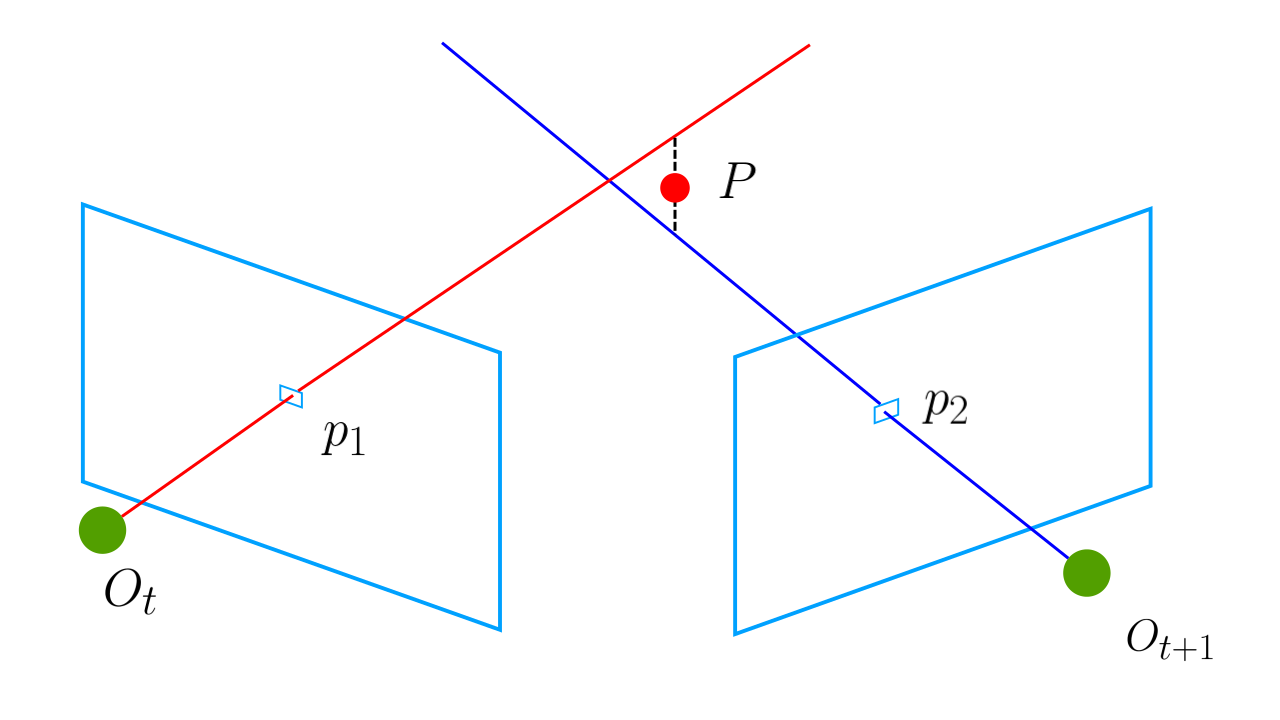
\includegraphics[width=0.9\linewidth]{vo1/triangularization}
	\caption{三角化获得地图点深度。}
	\label{fig:triangluar}
\end{figure}

三角测量是指,通过在不同位置在同一个路标点进行观察,从观察到的位置推断确定路标点的距离。三角测量最早由高斯提出并应用于测量学中,它在天文学、地理学的测量中都有应用。例如,我们可以通过不同季节观察到的星星的角度,估计它离我们的距离。在SLAM中,我们主要用三角化来估计像素点的距离。

和上一节类似,考虑图像$I_{1}$和$I_{2}$,以左图为参考,右图的变换矩阵为$\bm{T}$。相机光心为$O_{1}$和$O_{2}$。在$I_{1}$中有特征点$p_{1}$,对应$I_{2}$中有特征点$p_{2}$。理论上直线$O_{1}p_{1}$与$O_{2}p_{2}$在场景中会相交于一点$P$,该点即两个特征点所对应的地图点在三维场景中的位置。然而由于噪声的影响,这两条直线往往无法相交。因此,可以通过最二小乘法求解。

按照对极几何中的定义,设$\bm{x}_1, \bm{x}_2$为两个特征点的归一化坐标,那么它们满足:
\begin{equation}
s_2 \bm{x}_2 = s_1  \bm{R} \bm{x}_1 + \bm{t}.  
\end{equation}

现在已知$\bm{R}, \bm{t}$,我们想要求解两个特征点的深度$s_1, s_2$。从几何上看,可以在射线$O_1 p_1$上寻找3D点,使其投影位置接近$\bm{p}_2$,同理也可以在$O_2 p_2$上找,或者在两条线的中间。不同的策略对应着不同的计算方式,当然它们大同小异。比如,我们希望计算$s_1$,那么先对上式两侧左乘一个$\bm{x}_2^\wedge$,得:
\begin{equation}
\label{eq:x1tox2}
s_2 \bm{x}_2^\wedge \bm{x}_2 = 0 = s_1 \bm{x}_2^\wedge \bm{R} \bm{x}_1 + \bm{x}_2^\wedge \bm{t}. 
\end{equation}

该式左侧为零,右侧可看成$s_2$的一个方程,可以根据它直接求得$s_2$。有了$s_2$,$s_1$也非常容易求出。于是,我们就得到了两帧下的点的深度,确定了它们的空间坐标。当然,由于噪声的存在,我们估得的$\bm{R}, \bm{t}$不一定精确使式\eqref{eq:x1tox2}为零,所以更常见的做法是求最小二乘解而不是直接的解。

\section{实践:三角测量}
\subsection{三角测量代码}
下面,我们演示如何根据之前利用对极几何求解的相机位姿,通过三角化求出上一节特征点的空间位置。我们调用OpenCV提供的triangulation函数进行三角化。

\begin{lstlisting}[language=c++,caption=slambook2/ch7/triangulation.cpp(片段)]
void triangulation(
	const vector<KeyPoint> &keypoint_1,
	const vector<KeyPoint> &keypoint_2,
	const std::vector<DMatch> &matches,
	const Mat &R, const Mat &t,
	vector<Point3d> &points) {
	Mat T1 = (Mat_<float>(3, 4) <<
		1, 0, 0, 0,
		0, 1, 0, 0,
		0, 0, 1, 0);
	Mat T2 = (Mat_<float>(3, 4) <<
		R.at<double>(0, 0), R.at<double>(0, 1), R.at<double>(0, 2), t.at<double>(0, 0),
		R.at<double>(1, 0), R.at<double>(1, 1), R.at<double>(1, 2), t.at<double>(1, 0),
		R.at<double>(2, 0), R.at<double>(2, 1), R.at<double>(2, 2), t.at<double>(2, 0)
	);
	
	Mat K = (Mat_<double>(3, 3) << 520.9, 0, 325.1, 0, 521.0, 249.7, 0, 0, 1);
	vector<Point2f> pts_1, pts_2;
	for (DMatch m:matches) {
		// 将像素坐标转换至相机坐标
		pts_1.push_back(pixel2cam(keypoint_1[m.queryIdx].pt, K));
		pts_2.push_back(pixel2cam(keypoint_2[m.trainIdx].pt, K));
	}
	
	Mat pts_4d;
	cv::triangulatePoints(T1, T2, pts_1, pts_2, pts_4d);
	
	// 转换成非齐次坐标
	for (int i = 0; i < pts_4d.cols; i++) {
		Mat x = pts_4d.col(i);
		x /= x.at<float>(3, 0); // 归一化
		Point3d p(
			x.at<float>(0, 0),
			x.at<float>(1, 0),
			x.at<float>(2, 0)
		);
		points.push_back(p);
	}
}
\end{lstlisting}

同时,在main函数中加入三角测量部分,然后画出各点的深度示意图。读者可以自行运行此程序查看三角化结果。

\subsection{讨论}
关于三角测量,还有一个必须注意的地方。

三角测量是由\textbf{平移}得到的,有平移才会有对极几何中的三角形,才谈得上三角测量。因此,纯旋转是无法使用三角测量的,因为对极约束将永远满足。当然实际数据往往不会完全等于零。在平移存在的情况下,我们还要关心三角测量的不确定性,这会引出一个\textbf{三角测量的矛盾}。

如\autoref{fig:triangulation-discuss}~所示,当平移很小时,像素上的不确定性将导致较大的深度不确定性。也就是说,如果特征点运动一个像素$\delta x$,使得视线角变化了一个角度$\delta \theta$,那么将测量到深度值有$\delta d$的变化。从几何关系可以看到,当$\bm{t}$较大时,$\delta d$将明显变小,这说明平移较大时,在同样的相机分辨率下,三角化测量将更精确。对该过程的定量分析可以使用正弦定理得到。

因此,要提高三角化的精度,其一是提高特征点的提取精度,也就是提高图像分辨率——但这会导致图像变大,增加计算成本。另一方式是使平移量增大。但是,这会导致图像的\textbf{外观}发生明显的变化,比如箱子原先被挡住的侧面显示出来,或者物体的光照发生变化,等等。外观变化会使得特征提取与匹配变得困难。总而言之,增大平移,可能导致匹配失效;而平移太小,则三角化精度不够——这就是三角化的矛盾。我们把这个问题称为“视差”(parallax)。

\begin{figure}[!ht]
	\centering
	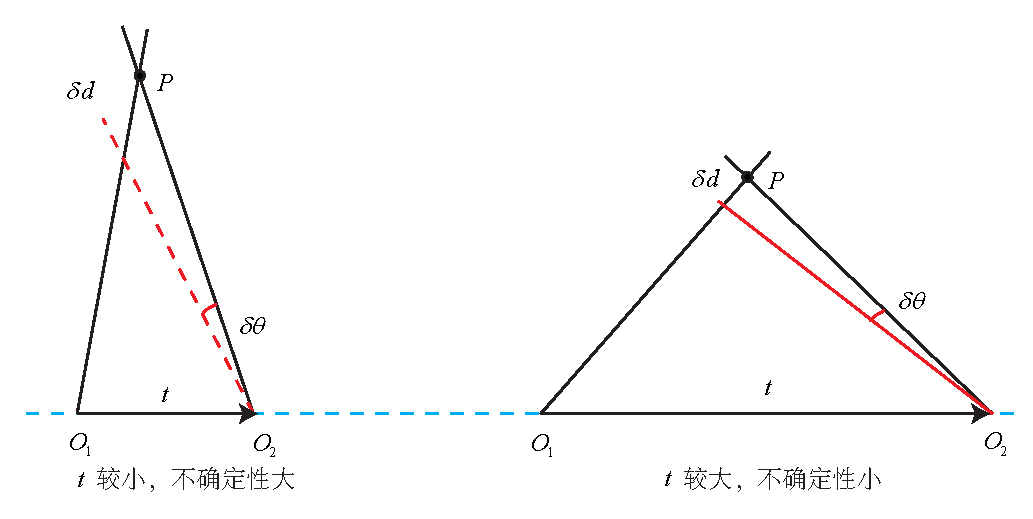
\includegraphics[width=1.0\linewidth]{vo1/triangulation-discuss.pdf}
	\caption{三角测量的矛盾。}
	\label{fig:triangulation-discuss}
\end{figure}

在单目视觉中,由于单目图像没有深度信息,我们要等待特征点被追踪几帧之后,产生了足够的视角,再用三角化来确定新增特征点的深度值。这个又时也被称为延迟三角化\textsuperscript{\cite{Davison2003}}。但是,如果相机发生了原地旋转,导致视差很小,那么就不好估计新观测到的特征点的深度。这种情况在机器人场合下更加常见,因为原地旋转往往是一个机器人常见的指令。在这种情况下,单目视觉就可能出现追踪失败、尺度不正确等情况。

虽然本节只介绍了三角化的深度估计,但只要我们愿意,也能够定量地计算每个特征点的\textbf{位置}及\textbf{不确定性}。所以,如果假设特征点服从高斯分布,并且不断地对它进行观测,在信息正确的情况下,我们就能够期望\textbf{它的方差会不断减小乃至收敛}。这就得到了一个\textbf{滤波器},称为\textbf{深度滤波器(Depth Filter)}。不过,由于它的原理较复杂,我们将留到后面再详细讨论它。下面,我们来讨论从3D−2D的匹配点来估计相机运动,以及3D−3D的估计方法。

\section{3D−2D:PnP}
PnP(Perspective-n-Point)是求解3D到2D点对运动的方法。它描述了当知道$n$个3D空间点及其投影位置时,如何估计相机的位姿。前面说到,2D−2D的对极几何方法需要8个或8个以上的点对(以八点法为例),且存在着初始化、纯旋转和尺度的问题。然而,如果两张图像中其中一张特征点的3D位置已知,那么最少只需3个点对(以及至少一个额外点验证结果)就可以估计相机运动。特征点的3D位置可以由三角化或者RGB-D相机的深度图确定。因此,在双目或RGB-D的视觉里程计中,我们可以直接使用PnP估计相机运动。而在单目视觉里程计中,必须先进行初始化,然后才能使用PnP。3D−2D方法不需要使用对极约束,又可以在很少的匹配点中获得较好的运动估计,是最重要的一种姿态估计方法。

PnP问题有很多种求解方法,例如,用3对点估计位姿的P3P\textsuperscript{\cite{GaoHouTangEtAl2003}}、直接线性变换(DLT)、EPnP(Efficient PnP)\textsuperscript{\cite{LepetitMoreno-NoguerFua2008}}、UPnP\textsuperscript{\cite{Penate-SanchezAndrade-CettoMoreno-Noguer2013}},等等。此外,还能用\textbf{非线性优化}的方式,构建最小二乘问题并迭代求解,也就是万金油式的Bundle Adjustment。我们先来看DLT,然后再讲解Bundle Adjustment。

\subsection{直接线性变换}
我们考虑这样一个问题:已知一组3D点的位置,以及它们在某个相机中的投影位置,求该相机的位姿。这个问题也可以用于求解给定地图和图像时的相机状态问题。如果把3D点看成在另一个相机坐标系中的点的话,也可以用来求解两个相机的相对运动问题。我们从简单的问题出发。

考虑某个空间点$P$,它的齐次坐标为${\bm{P}}=(X,Y,Z,1)^{\mathrm{T}}$。在图像$I_{1}$中,投影到特征点${\bm{x}}_{1}=(u_{1},v_{1},1)^{\mathrm{T}}$(以归一化平面齐次坐标表示)。此时相机的位姿$\bm{R}, \bm{t}$是未知的。与单应矩阵的求解类似,我们定义增广矩阵$[\bm{R}|\bm{t}]$为一个$3\times 4$的矩阵,包含了旋转与平移信息\footnote{请注意,这和$\mathrm{SE}(3)$中的变换矩阵$\bm{T}$是不同的。}。我们将其展开形式列写如下:
\begin{equation}
s
\begin{pmatrix}
u_{1} \\ v_{1} \\ 1
\end{pmatrix}
=
\begin{pmatrix}
t_{1} & t_{2} & t_{3} & t_{4}\\ 
t_{5} & t_{6} & t_{7} & t_{8}\\ 
t_{9} & t_{10} & t_{11} & t_{12}
\end{pmatrix}
\begin{pmatrix}
X \\ Y \\ Z \\ 1
\end{pmatrix}.
\end{equation}

用最后一行把$s$消去,得到两个约束:
\[
u_{1}=\frac{t_{1}X+t_{2}Y+t_{3}Z+t_{4}}{t_{9}X+t_{10}Y+t_{11}Z+t_{12}},\quad
v_{1}=\frac{t_{5}X+t_{6}Y+t_{7}Z+t_{8}}{t_{9}X+t_{10}Y+t_{11}Z+t_{12}}.
\]

为了简化表示,定义$\bm{T}$的行向量:
\[
\bm{t}_{1}=(t_{1},t_{2},t_{3},t_{4})^\mathrm{T},
\bm{t}_{2}=(t_{5},t_{6},t_{7},t_{8})^\mathrm{T},
\bm{t}_{3}=(t_{9},t_{10},t_{11},t_{12})^\mathrm{T},
\]
于是有:
\[
\bm{t}_1^\mathrm{T}\bm{P}-\bm{t}_3^\mathrm{T}\bm{P} u_1=0,
\]
和
\[
\bm{t}_2^\mathrm{T}\bm{P}-\bm{t}_3^\mathrm{T}\bm{P} v_1=0.
\]

请注意,$\bm{t}$是待求的变量,可以看到,每个特征点提供了两个关于$\bm{t}$的线性约束。假设一共有$N$个特征点,则可以列出如下线性方程组:
\begin{equation}
\begin{pmatrix}
\bm{P}_{1}^{\mathrm{T}} & 0 & -u_{1}\bm{P}_{1}^{\mathrm{T}}	\\
0 & \bm{P}_{1}^{\mathrm{T}} & -v_{1}\bm{P}_{1}^{\mathrm{T}}	\\
\vdots & \vdots & \vdots			\\
\bm{P}_{N}^{\mathrm{T}} & 0 & -u_{N}\bm{P}_{N}^{\mathrm{T}} \\
0 & \bm{P}_{N}^{\mathrm{T}} & -v_{N}\bm{P}_{N}^{\mathrm{T}}
\end{pmatrix}
\begin{pmatrix}
\bm{t}_{1} \\ \bm{t}_{2} \\ \bm{t}_{3}
\end{pmatrix}
=0.
\end{equation}

由于$\bm{t}$一共有12维,因此,最少通过6对匹配点即可实现矩阵$\bm{T}$的线性求解,这种方法称为直接线性变换(Direct Linear Transform,DLT)。当匹配点大于6对时,也可以使用SVD等方法对超定方程求最小二乘解。

在DLT求解中,我们直接将$\bm{T}$矩阵看成了12个未知数,忽略了它们之间的联系。因为旋转矩阵$\bm{R} \in \mathrm{SO}(3)$,用DLT求出的解不一定满足该约束,它是一个一般矩阵。平移向量比较好办,它属于向量空间。对于旋转矩阵$\bm{R}$,我们必须针对DLT估计的$\bm{T}$左边$3 \times 3$的矩阵块,寻找一个最好的旋转矩阵对它进行近似。这可以由QR分解完成\textsuperscript{\cite{Hartley2003, Chen1994}},也可以像这样来计算\textsuperscript{\cite{Barfoot2016,Green1952}}:
\begin{equation}
\bm{R} \leftarrow {\left( {\bm{R}{\bm{R}^\mathrm{T}}} \right)^{ - \frac{1}{2}}} \bm{R}.
\end{equation}
这相当于把结果从矩阵空间重新投影到$\mathrm{SE}(3)$流形上,转换成旋转和平移两部分。

需要解释的是,我们这里的$\bm{x}_1$使用了归一化平面坐标,去掉了内参矩阵$\bm{K}$的影响——这是因为内参$\bm{K}$在SLAM中通常假设为已知。即使内参未知,也能用PnP去估计$\bm{K}, \bm{R}, \bm{t}$三个量。然而由于未知量增多,效果会差一些。

\subsection{P3P}
下面讲的P3P是另一种解PnP的方法。它仅使用3对匹配点,对数据要求较少,因此这里也简单介绍一下(这部分推导借鉴了文献\cite{web:p3p})。

P3P需要利用给定的3个点的几何关系。它的输入数据为3对3D−2D匹配点。记3D点为$A, B, C$,2D点为$a,b,c$,其中小写字母代表的点为对应大写字母代表的点在相机成像平面上的投影,如\autoref{fig:p3p}~所示。此外,P3P还需要使用一对验证点,以从可能的解中选出正确的那一个(类似于对极几何情形)。记验证点对为$D-d$,相机光心为$O$。请注意,我们知道的是$A,B,C$在\textbf{世界坐标系中的坐标},而不是\textbf{在相机坐标系中的坐标}。一旦3D点在相机坐标系下的坐标能够算出,我们就得到了3D−3D的对应点,把PnP问题转换为了ICP问题。

\begin{figure}[!ht]
	\centering
	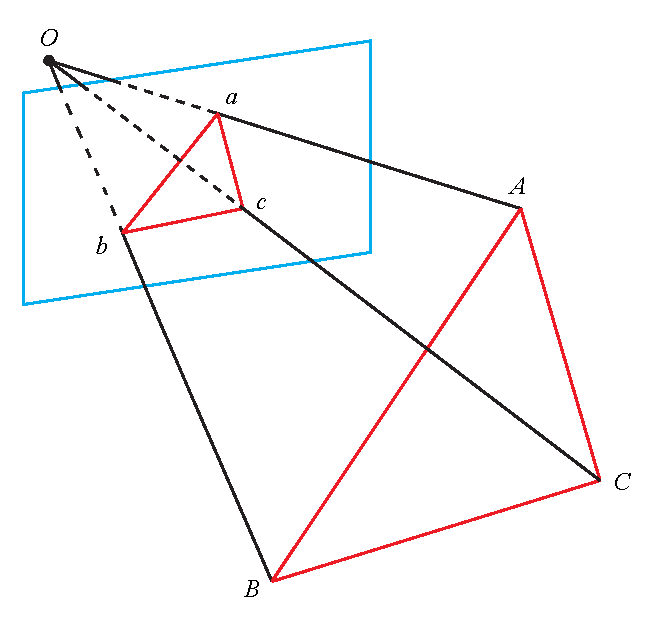
\includegraphics[width=0.54\linewidth]{vo1/p3p.pdf}
	\caption{P3P问题示意图。}
	\label{fig:p3p}
\end{figure}

首先,显然三角形之间存在对应关系:
\begin{equation}
\Delta Oab - \Delta OAB, \quad \Delta Obc - \Delta OBC, \quad \Delta Oac - \Delta OAC.
\end{equation}

来考虑$Oab$和$OAB$的关系。利用余弦定理,有:
\begin{equation}
O{A^2} + O{B^2} - 2OA \cdot OB \cdot \cos \left\langle a,b \right \rangle  = A{B^2}.
\end{equation}

对于其他两个三角形亦有类似性质,于是有:
\begin{equation}
\begin{array}{l}
O{A^2} + O{B^2} - 2OA \cdot OB \cdot \cos \left\langle a,b \right \rangle  = A{B^2}\\
O{B^2} + O{C^2} - 2OB \cdot OC \cdot \cos \left\langle b,c \right \rangle  = B{C^2}\\
O{A^2} + O{C^2} - 2OA \cdot OC \cdot \cos \left\langle a,c \right \rangle  = A{C^2}.
\end{array}
\end{equation}

对以上三式全体除以$OC^2$,并且记$x=OA/OC, y=OB/OC$,得:
\begin{equation}
\begin{array}{l}
{x^2} + {y^2} - 2xy\cos \left\langle a,b \right \rangle  = A{B^2}/O{C^2}\\
{y^2} + {1^2} - 2y\cos \left\langle b,c \right \rangle  = B{C^2}/O{C^2}\\
{x^2} + {1^2} - 2x\cos \left\langle a,c \right \rangle  = A{C^2}/O{C^2}.
\end{array}
\end{equation}

记$v = AB^2/OC^2, uv = BC^2/OC^2, wv = AC^2/OC^2$,有:
\begin{equation}
\begin{array}{l}
{x^2} + {y^2} - 2xy\cos \left\langle a,b \right \rangle  - v = 0\\
{y^2} + {1^2} - 2y\cos \left\langle b,c \right \rangle  - uv = 0\\
{x^2} + {1^2} - 2x\cos \left\langle a,c \right \rangle  - wv = 0.
\end{array}
\end{equation}

我们可以把第一个式子中的$v$放到等式一边,并代入其后两式,得:
\begin{equation}
\begin{array}{l}
\left( {1 - u} \right){y^2} - u{x^2} - \cos \left\langle b,c \right \rangle y + 2uxy\cos \left\langle a,b \right \rangle  + 1 = 0 \\
\left( {1 - w} \right){x^2} - w{y^2} - \cos \left\langle a,c \right \rangle x + 2wxy\cos \left\langle a,b \right \rangle  + 1 = 0.
\end{array}
\end{equation}

注意这些方程中的已知量和未知量。由于我们知道2D点的图像位置,3个余弦角$\cos \left \langle a,b \right \rangle$, $\cos \left\langle b,c \right \rangle$, $\cos \left\langle a,c \right \rangle$是已知的。同时,$u=BC^2/AB^2, w=AC^2/AB^2$可以通过$A,B,C$在世界坐标系下的坐标算出,变换到相机坐标系下之后,这个比值并不改变。该式中的$x,y$是未知的,随着相机移动会发生变化。因此,该方程组是关于$x,y$的一个二元二次方程(多项式方程)。解析地求解该方程组是一个复杂的过程,需要用吴消元法。这里不展开对该方程解法的介绍,感兴趣的读者请参阅文献\cite{GaoHouTangEtAl2003}。类似于分解$\bm{E}$的情况,该方程最多可能得到4个解,但我们可以用验证点来计算最可能的解,得到$A,B,C$在相机坐标系下的3D坐标。然后,根据3D−3D的点对,计算相机的运动$\bm{R}, \bm{t}$。这部分将在7.9节介绍。

从P3P的原理可以看出,为了求解PnP,我们利用了三角形相似性质,求解投影点$a,b,c$在相机坐标系下的3D坐标,最后把问题转换成一个3D到3D的位姿估计问题。在后文将看到,带有匹配信息的3D−3D位姿求解非常容易,所以这种思路是非常有效的。其他的一些方法,例如EPnP,亦采用了这种思路。然而,P3P也存在着一些问题:

\begin{enumerate}
	\item P3P只利用3个点的信息。当给定的配对点多于3组时,难以利用更多的信息。
	\item 如果3D点或2D点受噪声影响,或者存在误匹配,则算法失效。
\end{enumerate}

所以后续人们还提出了许多别的方法,如EPnP、UPnP等。它们利用更多的信息,而且用迭代的方式对相机位姿进行优化,以尽可能地消除噪声的影响。不过,相对于P3P来说,原理会更加复杂一些,所以我们建议读者阅读原始的论文,或通过实践来理解PnP过程。在SLAM当中,通常的做法是先使用P3P/EPnP等方法估计相机位姿,然后构建最小二乘优化问题对估计值进行调整(Bundle Adjustment)。在相机运动足够连续时,也可以假设相机不动或匀速运动,用推测值作为初始值进行优化。接下来我们从非线性优化角度来看一下PnP问题。

%
%\subsubsection{随机采样一致(RANSAC)}
%特征匹配的环节会不可避免地出现大量的错误匹配,它们将严重影响之后姿态估计的准确度,因此我们需要设法把错误的匹配剔除。下面以八点法计算基础矩阵为例,讲解RANSAC如何执行,基础矩阵的意义与推导,及八点法将在本书的第\ref{sec:funmatrix}节进行详细讲解。\par
%
%\begin{enumerate}
%	\item 随机在所有匹配点对中抽取8对,设为组$M_{k}$,$k=1,2,...,K$。
%	\item 使用组$M_{k}$,使用八点法计算相应的基础矩阵,$F_{k}$。
%	\item 对于当前的每一个内点点对$In_{i}$,$i=1,2,...,I$, 计算$F_{k}$的重投影误差$e_{k}$ (关于重投影误差请参阅本书第\ref{sec:reprojection}节)。若$e_{k}^{i}$小于指定阈值$threshold$,则判断该点对有效,对$F_{k}^{i}$的评分为$score_{k}^{i}=\frac{1}{e_{k}^{i}}$。否则将该点对从内点点对中剔除。最终对$F_{k}$的评分$score_{k}$就是所有有效点评分$score_{k}^{i}$之和。
%	\item 重复1,2,3步,直到达到最大的迭代次数$MaxIteration$,该值手动设定。最终要取的8对匹配点就是评分最高的$F_{k}$所对应的组$M_{k}$。
%\end{enumerate}
%
%
%事实上RANSAC是一种算法思想,对于不同的模型,有不同的参数及评价标准。如上述例子中是基础矩阵,参数是8对匹配点,而评价标准是最小化重投影误差。理论上迭代次数越大,越有可能找到模型的最佳参数。但是由于SLAM中实时性的需要,我们需要在找到合理模型参数的情况下,迭代次数最少。假设$u$是找到一组内点的概率,$v=1-u$是找到一组外点的概率,$p$是至少有一组参数不包含外点的概率(通常设为$99\%$),$m$为所需的参数数量,$N$为迭代次数。则有:
%
%\begin{equation}
%1-p=(1-u^{m})^{N}
%\end{equation}
%
%所以最小迭代次数可以由以下式子找出,$u$和$v$通常使用经验值。
%
%\begin{equation}
%N=\frac{log(1-p)}{1-(1-v)^{m}}
%\end{equation}


\subsection{最小化重投影误差求解PnP}
\label{sec:BA-vo1}
除了使用线性方法之外,我们还可以把PnP问题构建成一个关于重投影误差的非线性最小二乘问题。这将用到本书第\ref{cpt:4}讲和第\ref{cpt:5}讲的知识。前面说的线性方法,往往是\textbf{先求相机位姿,再求空间点位置},而非线性优化则是把它们都看成优化变量,放在一起优化。这是一种非常通用的求解方式,我们可以用它对PnP或ICP给出的结果进行优化。这一类\textbf{把相机和三维点放在一起进行最小化}的问题,统称为Bundle Adjustment(光束法平差),简称为BA\footnote{需要说明的是,BA在不同文献、语境下的意义并不完全一致。有些学者仅把最小化重投影误差的问题称为BA,而另一些学者的BA概念更加宽泛一些,即使这个BA只有一个相机,或加入了其他类似的传感器,可以都称为BA。我个人更喜欢宽泛一些的BA概念,所以在这里计算PnP的方法也称为BA。}。

我们完全可以在PnP中构建一个Bundle Adjustment问题对相机位姿进行优化。如果相机是连续运动的(比如大多数SLAM过程),也可以直接用BA求解相机位姿。我们将在本节给出此问题在两个视图下的基本形式,然后在第9讲讨论较大规模的BA问题。

考虑$n$个三维空间点$P$及其投影$p$,我们希望计算相机的位姿$\bm{R}, \bm{t}$,它的李群表示为$\bm{T}$。假设某空间点坐标为$\bm{P}_i=[X_i,Y_i,Z_i]^\mathrm{T}$,其投影的像素坐标为$\bm{u}_i=[u_i,v_i]^\mathrm{T}$。根据第\ref{cpt:5}讲的内容,像素位置与空间点位置的关系如下:
\begin{equation}
s_i \left[ 
\begin{array}{l}
u_i \\ v_i \\ 1
\end{array}
\right] = \bm{K} \bm{T} \left[ 
\begin{array}{l}
X_i \\ Y_i \\ Z_i \\ 1
\end{array} \right]  .
\end{equation}
写成矩阵形式就是:
\[
{{s_i {\bm{u}}_i} = \bm{K} \bm{T} \bm{P}}_i.
\]

这个式子隐含了一次从齐次坐标到非齐次的转换,否则按矩阵的乘法来说,维度是不对的\footnote{ $ \bm{T} {\bm{P}_i}$结果是$4 \times 1$的,而其左侧的$\bm{K}$是$3 \times 3$的,所以必须把$\bm{T}\bm{P}_i$的前三维取出来,变成三维的非齐次坐标。或者,用$\bm{R}\bm{P}+\bm{t}$亦无不可。}。现在,由于相机位姿未知及观测点的噪声,该等式存在一个误差。因此,我们把误差求和,构建最小二乘问题,然后寻找最好的相机位姿,使它最小化:
\begin{equation}
{\bm{T}^*} = \arg \mathop {\min }\limits_{\bm{T}}  \frac{1}{2}\sum\limits_{i = 1}^n {\left\| {{{\bm{u}}_i} - \frac{1}{s_i} \bm{K}\bm{T}{\bm{P}}_i} \right\|_2^2} .
\end{equation}

该问题的误差项,是将3D点的投影位置与观测位置作差,所以称为\textbf{重投影误差}。使用齐次坐标时,这个误差有3维。不过,由于${\bm{u}}$最后一维为1,该维度的误差一直为零,因而我们更多时候使用非齐次坐标,于是误差就只有2维了。如\autoref{fig:reprojection}~所示,我们通过特征匹配知道了$p_1$和$p_2$是同一个空间点$P$的投影,但是不知道相机的位姿。在初始值中,$P$的投影$\hat{p}_2$与实际的$p_2$之间有一定的距离。于是我们调整相机的位姿,使得这个距离变小。不过,由于这个调整需要考虑很多个点,所以最后的效果是整体误差的缩小,而每个点的误差通常都不会精确为零。

\begin{figure}[!htp]
	\centering
	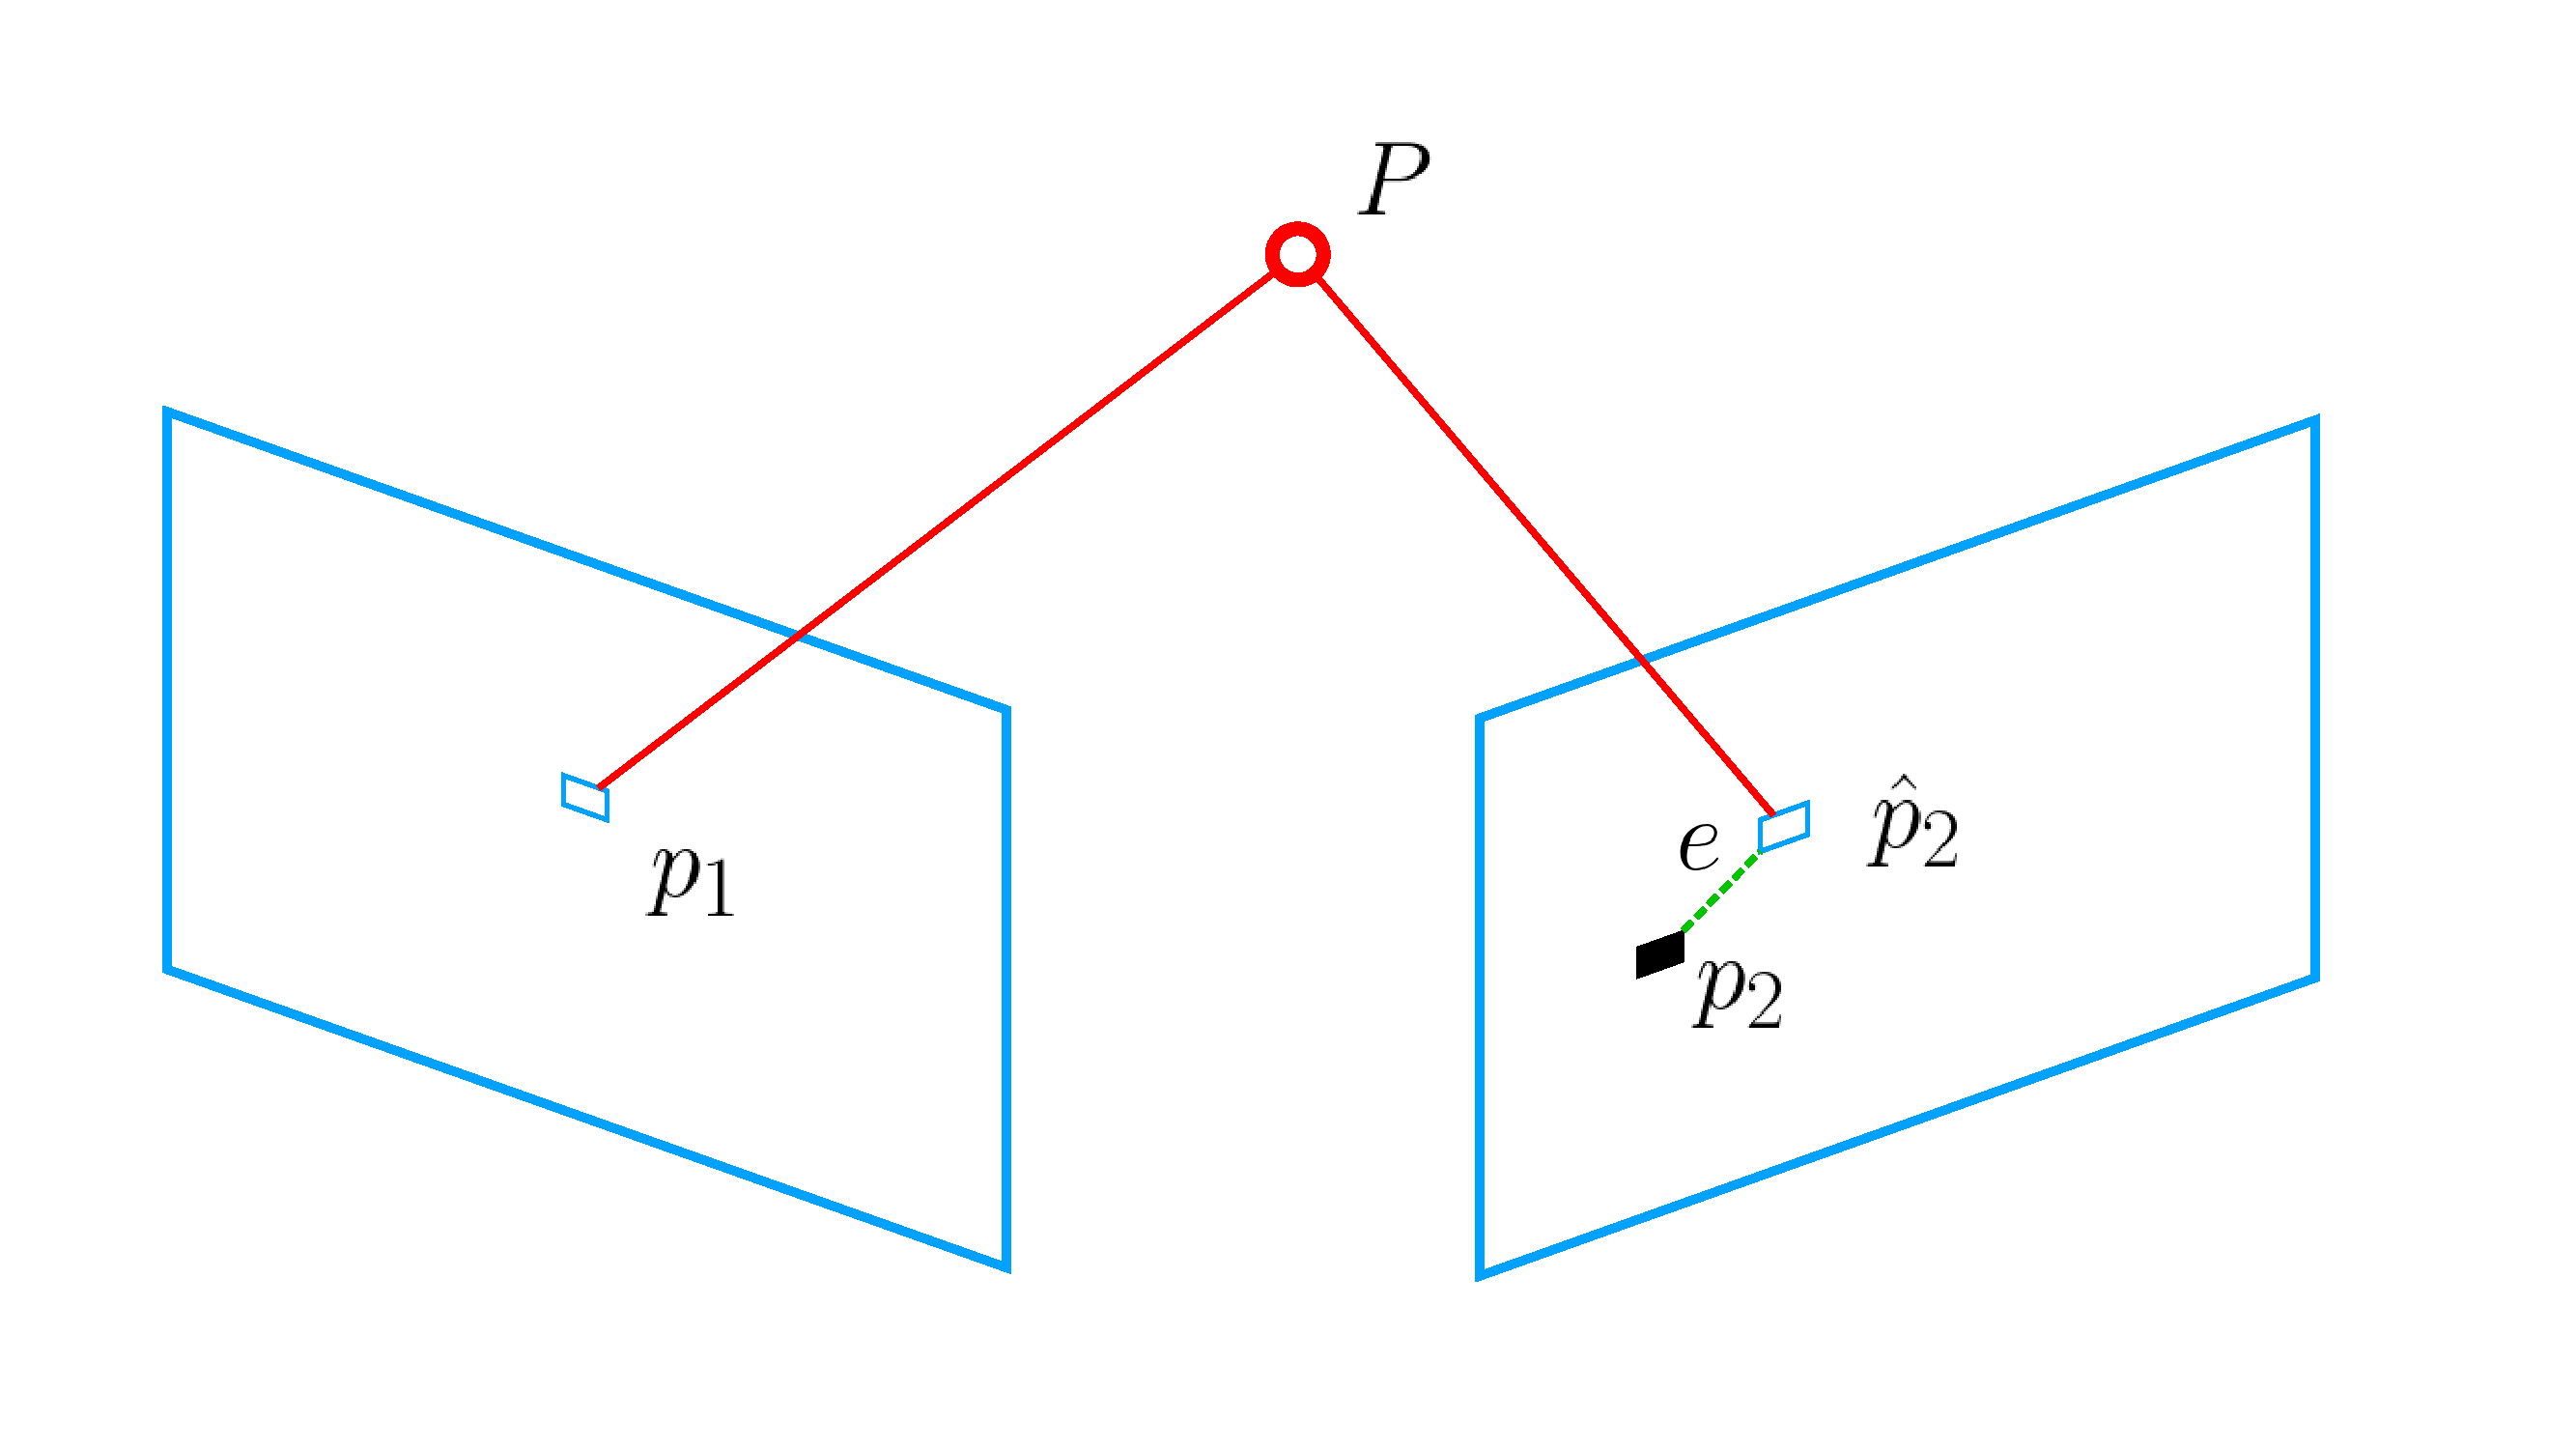
\includegraphics[width=0.8\linewidth]{vo1/reprojection}
	\caption{重投影误差示意图。}
	\label{fig:reprojection}
\end{figure}

最小二乘优化问题已经在第\ref{cpt:6}讲介绍过了。使用李代数,可以构建无约束的优化问题,很方便地通过高斯牛顿法、列文伯格—马夸尔特方法等优化算法进行求解。不过,在使用高斯牛顿法和列文伯格—马夸尔特方法之前,我们需要知道每个误差项关于优化变量的导数,也就是\textbf{线性化}:
\begin{equation}
\bm{e}( \bm{x} + \Delta \bm{x} ) \approx \bm{e}(\bm{x}) + \bm{J} ^\mathrm{T}\Delta \bm{x}.
\end{equation}

这里的$\bm{J}^\mathrm{T}$的形式是值得讨论的,甚至可以说是关键所在。我们固然可以使用数值导数,但如果能够推导出解析形式,则优先考虑解析导数。现在,当$\bm{e}$为像素坐标误差(2维),$\bm{x}$为相机位姿(6维)时,$\bm{J}^\mathrm{T}$将是一个$2 \times 6$的矩阵。我们来推导$\bm{J}^\mathrm{T}$的形式。

回忆李代数的内容,我们介绍了如何使用扰动模型来求李代数的导数。首先,记变换到相机坐标系下的空间点坐标为$\bm{P}'$,并且将其前3维取出来:
\begin{equation}
\bm{P}' = \left( \bm{T}{\bm{P}} \right)_{1:3}= [X', Y', Z']^\mathrm{T}.
\end{equation}

那么,相机投影模型相对于$\bm{P}'$为
\begin{equation}
s {\bm{u}} = \bm{K} \bm{P}'.
\end{equation}

展开:
\begin{equation}
\left[ \begin{array}{l}
su\\
sv\\
s
\end{array} \right] = \left[ {\begin{array}{*{20}{c}}
	{{f_x}}&0&{{c_x}}\\
	0&{{f_y}}&{{c_y}}\\
	0&0&1
	\end{array}} \right]\left[ \begin{array}{l}
X'\\
Y'\\
Z'
\end{array} \right].
\end{equation}

利用第3行消去$s$(实际上就是$\bm{P}'$的距离),得:
\begin{equation}
\label{eq:uv2xyz}
u = {f_x}\frac{{X'}}{{Z'}} + {c_x}, \quad v = {f_y}\frac{{Y'}}{{Z'}} + {c_y}.
\end{equation}

这与第\ref{cpt:5}讲的相机模型是一致的。当我们求误差时,可以把这里的$u,v$与实际的测量值比较,求差。在定义了中间变量后,我们对$\bm{T}$左乘扰动量$\delta \boldsymbol{\xi}$,然后考虑$\bm{e}$的变化关于扰动量的导数。利用链式法则,可以列写如下:
\begin{equation}
\frac{{\partial \bm{e}}}{{\partial \delta \boldsymbol{\xi} }} = \mathop {\lim }\limits_{\delta \boldsymbol{\xi}  \to 0} \frac{{\bm{e}\left( {\delta \boldsymbol{\xi}  \oplus \boldsymbol{\xi} } \right)-\bm{e}(\boldsymbol{\xi})}}{{\delta \boldsymbol{\xi} }}  = \frac{{\partial \bm{e}}}{{\partial \bm{P}'}}\frac{{\partial \bm{P}'}}{{\partial \delta \boldsymbol{\xi} }}.
\end{equation}

这里的$\oplus$指李代数上的左乘扰动。第一项是误差关于投影点的导数,在式\eqref{eq:uv2xyz}已经列出了变量之间的关系,易得:
\begin{equation}
\frac{{\partial \bm{e}}}{{\partial \bm{P}'}} = -\left[ 
{\begin{array}{*{20}{c}}
	{\frac{{\partial u}}{{\partial X'}}}&{\frac{{\partial u}}{{\partial Y'}}}&{\frac{{\partial u}}{{\partial Z'}}}\\
	{\frac{{\partial v}}{{\partial X'}}}&{\frac{{\partial v}}{{\partial Y'}}}&{\frac{{\partial v}}{{\partial Z'}}}
	\end{array}} \right] 
= - \left[ {\begin{array}{*{20}{c}}
	{\frac{{{f_x}}}{Z'}}&0&{ - \frac{{{f_x}X'}}{{{Z'^2}}}}\\
	0&{\frac{{{f_y}}}{Z'}}&{ - \frac{{{f_y}Y'}}{Z'^2}}
\end{array}} \right].
\end{equation}

而第二项为变换后的点关于李代数的导数,根据\ref{sec:se3-diff}节中的推导,得:
\begin{equation}
\frac{{\partial \left( \bm{TP} \right)}}{{\partial \delta \boldsymbol{\xi} }} = {\left( \bm{TP} \right)^ \odot } = \left[ 
\begin{array}{*{20}{cc}}
\bm{I} &- \bm{P}'^ \wedge \\
\bm{0}^\mathrm{T} &\bm{0}^\mathrm{T} 
\end{array}
\right].
\end{equation}

而在$\bm{P}'$的定义中,我们取出了前3维,于是得:
\begin{equation}
\frac{{\partial \bm{P}'}}{{\partial \delta \boldsymbol{\xi} }} = \left[ { \bm{I}, - {\bm{P}'^ \wedge }} \right].
\end{equation}

将这两项相乘,就得到了$2 \times 6$的雅可比矩阵:
\begin{equation}
\label{eq:jacob-uv2xi}
\frac{{\partial \bm{e}}}{{\partial \delta \boldsymbol{\xi} }} = - \left[ {\begin{array}{*{20}{c}}
	{\frac{{{f_x}}}{Z'}}&0&{ - \frac{{{f_x}X'}}{{{Z'^2}}}}&{ - \frac{{{f_x}X'Y'}}{{{Z'^2}}}}&{{f_x} + \frac{{{f_x}{X'^2}}}{{{Z'^2}}}}&{ - \frac{{{f_x}Y'}}{Z'}}\\
	0&{\frac{{{f_y}}}{Z'}}&{ - \frac{{{f_y}Y'}}{{{Z'^2}}}}&{ - {f_y} - \frac{{{f_y}{Y'^2}}}{{{Z'^2}}}}&{\frac{{{f_y}X'Y'}}{{{Z'^2}}}}&{\frac{{{f_y}X'}}{Z'}}
	\end{array}} \right].
\end{equation}

这个雅可比矩阵描述了重投影误差关于相机位姿李代数的一阶变化关系。我们保留了前面的负号,这是因为误差是由\textbf{观测值减预测值}定义的。它当然也可反过来,定义成“预测值减观测值”的形式。在那种情况下,只要去掉前面的负号即可。此外,如果$\mathfrak{se}(3)$的定义方式是旋转在前,平移在后,只要把这个矩阵的前3列与后3列对调即可。

另一方面,除了优化位姿,我们还希望优化特征点的空间位置。因此,需要讨论$\bm{e}$关于空间点$\bm{P}$的导数。所幸这个导数矩阵相对来说容易一些。仍利用链式法则,有:
\begin{equation}
\frac{{\partial \bm{e}}}{{\partial \bm{P} }} = \frac{{\partial \bm{e}}}{{\partial \bm{P}'}}\frac{{\partial \bm{P}'}}{{\partial \bm{P} }}.
\end{equation}

第一项在前面已推导,关于第二项,按照定义
\[
\bm{P}'= (\bm{T} \bm{P})_{1:3} = \bm{R} \bm{P} + \bm{t},
\]
我们发现$\bm{P}'$对$\bm{P}$求导后将只剩下$\bm{R}$。于是:
\begin{equation}
\label{eq:jacob-uv2P}
\frac{{\partial \bm{e}}}{{\partial \bm{P} }} = -\left[ 
\begin{array}{*{20}{c}}
	\frac{f_x}{Z'} & 0 &- \frac{f_x X'}{Z'^2} \\
	0 & \frac{f_y}{Z'} & - \frac{f_y Y'}{Z'^2}
\end{array} \right] \bm{R}.
\end{equation}

于是,我们推导出了观测相机方程关于相机位姿与特征点的两个导数矩阵。它们\textbf{十分重要},能够在优化过程中提供重要的梯度方向,指导优化的迭代。

\section{实践:求解PnP}
\subsection{使用EPnP求解位姿}
下面,我们通过实验理解一下PnP的过程。首先,我们演示如何使用OpenCV的EPnP求解PnP问题,然后通过非线性优化再次求解。在第二版书中,我们将增加一个手写优化的实验。由于PnP需要使用3D点,为了避免初始化带来的麻烦,我们使用了RGB-D相机中的深度图(1_depth.png)作为特征点的3D位置。首先来看OpenCV提供的PnP函数:

\begin{lstlisting}[language=c++,caption=slambook2/ch7/pose_estimation_3d2d.cpp(片段)]
int main( int argc, char** argv ) {
    Mat r, t;
   solvePnP(pts_3d, pts_2d, K, Mat(), r, t, false); // 调用OpenCV 的 PnP 求解,可选择EPNP,DLS等方法
   Mat R;
   cv::Rodrigues(r, R); // r为旋转向量形式,用Rodrigues公式转换为矩阵
   cout << "R=" << endl << R << endl;
   cout << "t=" << endl << t << endl;
}
\end{lstlisting}

在例程中,得到配对特征点后,我们在第一个图的深度图中寻找它们的深度,并求出空间位置。以此空间位置为3D点,再以第二个图像的像素位置为2D点,调用EPnP求解PnP问题。程序输出如下:

\begin{lstlisting}[language=sh,caption=终端输入:]
% build/pose_estimation_3d2d 1.png 2.png d1.png d2.png
-- Max dist : 95.000000 
-- Min dist : 4.000000 
一共找到了79组匹配点
3d-2d pairs: 76
R=
[0.9978662025826269, -0.05167241613316376, 0.03991244360207524;
0.0505958915956335, 0.998339762771668, 0.02752769192381471;
-0.04126860182960625, -0.025449547736074, 0.998823919929363]
t=
[-0.1272259656955879;
-0.007507297652615337;
0.06138584177157709]
\end{lstlisting}

读者可以对比先前2D−2D情况下求解的$\bm{R},\bm{t}$看看有什么不同。可以看到,在有3D信息时,估计的$\bm{R}$几乎是相同的,而$\bm{t}$相差得较多。这是由于引入了新的深度信息所致。不过,由于Kinect采集的深度图本身会有一些误差,所以这里的3D点也不是准确的。在较大规模的BA中,我们会希望把位姿和所有三维特征点同时优化。


\subsection{手写位姿估计}
下面演示如何使用非线性优化的方式计算相机位姿。我们先手写一个高斯牛顿法的PnP,然后再演示如何调用g2o来求解。  
\begin{lstlisting}[language=c++,caption=slambook2/ch7/pose_estimation_3d2d.cpp(片段)]
void bundleAdjustmentGaussNewton(
const VecVector3d &points_3d,
const VecVector2d &points_2d,
const Mat &K,
Sophus::SE3d &pose) {
	typedef Eigen::Matrix<double, 6, 1> Vector6d;
	const int iterations = 10;
	double cost = 0, lastCost = 0;
	double fx = K.at<double>(0, 0);
	double fy = K.at<double>(1, 1);
	double cx = K.at<double>(0, 2);
	double cy = K.at<double>(1, 2);
	
	for (int iter = 0; iter < iterations; iter++) {
		Eigen::Matrix<double, 6, 6> H = Eigen::Matrix<double, 6, 6>::Zero();
		Vector6d b = Vector6d::Zero();
		
		cost = 0;
		// compute cost
		for (int i = 0; i < points_3d.size(); i++) {
			Eigen::Vector3d pc = pose * points_3d[i];
			double inv_z = 1.0 / pc[2];
			double inv_z2 = inv_z * inv_z;
			Eigen::Vector2d proj(fx * pc[0] / pc[2] + cx, fy * pc[1] / pc[2] + cy);
			Eigen::Vector2d e = points_2d[i] - proj;
			cost += e.squaredNorm();
			Eigen::Matrix<double, 2, 6> J;
			J << -fx * inv_z,
			0,
			fx * pc[0] * inv_z2,
			fx * pc[0] * pc[1] * inv_z2,
			-fx - fx * pc[0] * pc[0] * inv_z2,
			fx * pc[1] * inv_z,
			0,
			-fy * inv_z,
			fy * pc[1] * inv_z,
			fy + fy * pc[1] * pc[1] * inv_z2,
			-fy * pc[0] * pc[1] * inv_z2,
			-fy * pc[0] * inv_z;
			
			H += J.transpose() * J;
			b += -J.transpose() * e;
		}
		
		Vector6d dx;
		dx = H.ldlt().solve(b);
		
		if (isnan(dx[0])) {
			cout << "result is nan!" << endl;
			break;
		}
		
		if (iter > 0 && cost >= lastCost) {
			// cost increase, update is not good
			cout << "cost: " << cost << ", last cost: " << lastCost << endl;
			break;
		}
		
		// update your estimation
		pose = Sophus::SE3d::exp(dx) * pose;
		lastCost = cost;
		
		cout << "iteration " << iter << " cost=" << cout.precision(12) << cost << endl;
		if (dx.norm() < 1e-6) {
			// converge
			break;
		}
	}
	
	cout << "pose by g-n: \n" << pose.matrix() << endl;
}
\end{lstlisting}

在这个小函数中,我们根据前面的理论推导,实现一个简单的高斯牛顿迭代优化。之后我们将比较OpenCV、手写实现和g2o实现之间的效率差异。

\subsection{使用g2o进行BA优化}
在手写了一遍优化流程之后,我们再来看如何用g2o实现同样的操作(事实上用Ceres也完全类似)。g2o的基本知识在第\ref{cpt:6}讲中已经介绍过了。在使用g2o之前,我们要把问题建模成一个图优化问题,如\autoref{fig:ba-graph}~所示。

\begin{figure}[!htp]
	\centering
	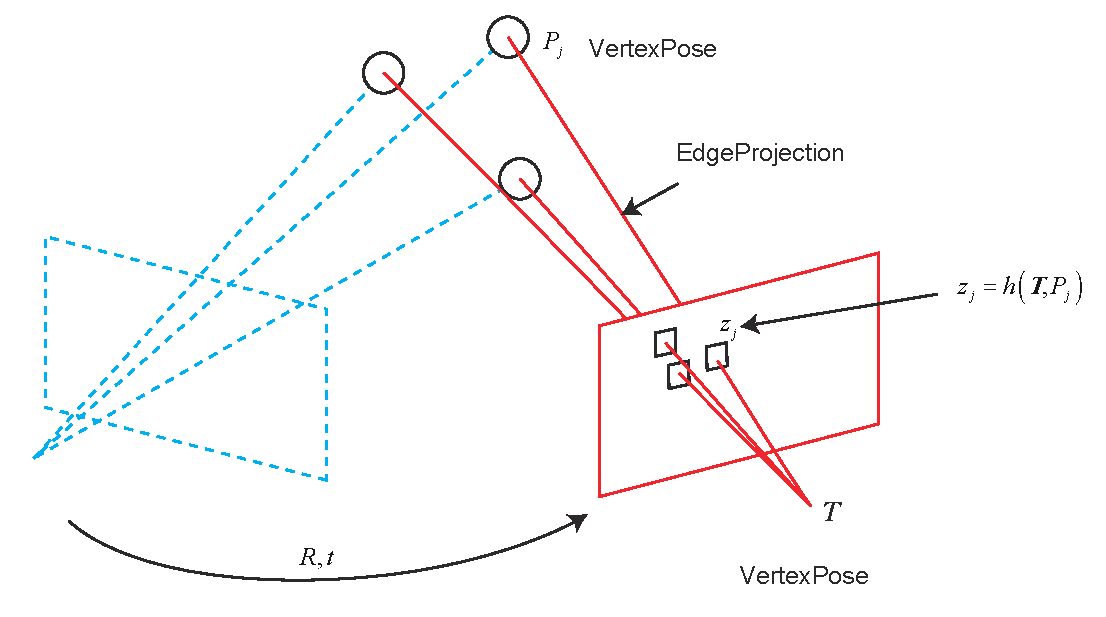
\includegraphics[width=0.9\linewidth]{vo1/ba-graph}
	\caption{PnP的Bundle Adjustment的图优化表示。}
	\label{fig:ba-graph}
\end{figure}

在这个图优化中,节点和边的选择如下:
\begin{enumerate}
	\item \textbf{节点}:第二个相机的位姿节点$\bm{T} \in \mathrm{SE}(3)$。
	\item \textbf{边}:每个3D点在第二个相机中的投影,以观测方程来描述:
	\[
	\bm{z}_j = h(\bm{T}, \bm{P}_{j}).
	\]
\end{enumerate}

由于第一个相机位姿固定为零,我们没有把它写到优化变量里,但在更多的场合里,我们会考虑更多相机的估计。现在我们根据一组3D点和第二个图像中的2D投影,估计第二个相机的位姿。所以我们把第一个相机画成虚线,表明不希望考虑它。

g2o提供了许多关于BA的节点和边,例如g2o/\\types/sba/types\_six\_dof\_expmap.h中提供了李代数表达的节点和边。在第二版书中,我们自己实现一个VertexPose顶点和EdgeProjection边,如下:
\begin{lstlisting}[language=c++,caption=slambook2/ch7/pose_estimation_3d2d.cpp(片段)]
/// vertex and edges used in g2o ba
class VertexPose : public g2o::BaseVertex<6, Sophus::SE3d> {
	public:
	EIGEN_MAKE_ALIGNED_OPERATOR_NEW;
	
	virtual void setToOriginImpl() override {
		_estimate = Sophus::SE3d();
	}
	
	/// left multiplication on SE3
	virtual void oplusImpl(const double *update) override {
		Eigen::Matrix<double, 6, 1> update_eigen;
		update_eigen << update[0], update[1], update[2], update[3], update[4], update[5];
		_estimate = Sophus::SE3d::exp(update_eigen) * _estimate;
	}
	
	virtual bool read(istream &in) override {}
	
	virtual bool write(ostream &out) const override {}
};

class EdgeProjection : public g2o::BaseUnaryEdge<2, Eigen::Vector2d, VertexPose> {
	public:
	EIGEN_MAKE_ALIGNED_OPERATOR_NEW;
	
	EdgeProjection(const Eigen::Vector3d &pos, const Eigen::Matrix3d &K) : _pos3d(pos), _K(K) {}
	
	virtual void computeError() override {
		const VertexPose *v = static_cast<VertexPose *> (_vertices[0]);
		Sophus::SE3d T = v->estimate();
		Eigen::Vector3d pos_pixel = _K * (T * _pos3d);
		pos_pixel /= pos_pixel[2];
		_error = _measurement - pos_pixel.head<2>();
	}
	
	virtual void linearizeOplus() override {
		const VertexPose *v = static_cast<VertexPose *> (_vertices[0]);
		Sophus::SE3d T = v->estimate();
		Eigen::Vector3d pos_cam = T * _pos3d;
		double fx = _K(0, 0);
		double fy = _K(1, 1);
		double cx = _K(0, 2);
		double cy = _K(1, 2);
		double X = pos_cam[0];
		double Y = pos_cam[1];
		double Z = pos_cam[2];
		double Z2 = Z * Z;
		_jacobianOplusXi
		<< -fx / Z, 0, fx * X / Z2, fx * X * Y / Z2, -fx - fx * X * X / Z2, fx * Y / Z,
		0, -fy / Z, fy * Y / (Z * Z), fy + fy * Y * Y / Z2, -fy * X * Y / Z2, -fy * X / Z;
	}
	
	virtual bool read(istream &in) override {}
	
	virtual bool write(ostream &out) const override {}
	
	private:
	Eigen::Vector3d _pos3d;
	Eigen::Matrix3d _K;
};
\end{lstlisting}

这里实现了顶点的更新和边的误差计算。下面就是将它们组成一个图优化问题:
\begin{lstlisting}[language=c++,caption=slambook2/ch7/pose_estimation_3d2d.cpp(片段)]
void bundleAdjustmentG2O(
const VecVector3d &points_3d,
const VecVector2d &points_2d,
const Mat &K,
Sophus::SE3d &pose) {
	// 构建图优化,先设定g2o
	typedef g2o::BlockSolver<g2o::BlockSolverTraits<6, 3>> BlockSolverType;  // pose is 6, landmark is 3
	typedef g2o::LinearSolverDense<BlockSolverType::PoseMatrixType> LinearSolverType; // 线性求解器类型
	// 梯度下降方法,可以从GN, LM, DogLeg 中选
	auto solver = new g2o::OptimizationAlgorithmsGaussNewton(
		g2o::make_unique<BlockSolverType>(g2o::make_unique<LinearSolverType>()));
	g2o::SparseOptimizer optimizer;     // 图模型
	optimizer.setAlgorithm(solver);   // 设置求解器
	optimizer.setVerbose(true);       // 打开调试输出
	
	// vertex
	VertexPose *vertex_pose = new VertexPose(); // camera vertex_pose
	vertex_pose->setId(0);
	vertex_pose->setEstimate(Sophus::SE3d());
	optimizer.addVertex(vertex_pose);
	
	// K
	Eigen::Matrix3d K_eigen;
	K_eigen <<
	K.at<double>(0, 0), K.at<double>(0, 1), K.at<double>(0, 2),
	K.at<double>(1, 0), K.at<double>(1, 1), K.at<double>(1, 2),
	K.at<double>(2, 0), K.at<double>(2, 1), K.at<double>(2, 2);
	
	// edges
	int index = 1;
	for (size_t i = 0; i < points_2d.size(); ++i) {
		auto p2d = points_2d[i];
		auto p3d = points_3d[i];
		EdgeProjection *edge = new EdgeProjection(p3d, K_eigen);
		edge->setId(index);
		edge->setVertex(0, vertex_pose);
		edge->setMeasurement(p2d);
		edge->setInformation(Eigen::Matrix2d::Identity());
		optimizer.addEdge(edge);
		index++;
	}
	
	chrono::steady_clock::time_point t1 = chrono::steady_clock::now();
	optimizer.setVerbose(true);
	optimizer.initializeOptimization();
	optimizer.optimize(10);
	chrono::steady_clock::time_point t2 = chrono::steady_clock::now();
	chrono::duration<double> time_used = chrono::duration_cast<chrono::duration<double>>(t2 - t1);
	cout << "optimization costs time: " << time_used.count() << " seconds." << endl;
	cout << "pose estimated by g2o =\n" << vertex_pose->estimate().matrix() << endl;
	pose = vertex_pose->estimate();
}
\end{lstlisting}

程序大体上和第6讲的g2o类似。我们首先声明了g2o图优化器,并配置优化求解器和梯度下降方法。然后根据估计到的特征点,将位姿和空间点放到图中。最后调用优化函数进行求解。最后,运行的部分输出如下:

\begin{lstlisting}[language=sh,caption=终端输入:]
./build/pose_estimation_3d2d 1.png 2.png 1_depth.png 2_depth.png
-- Max dist : 95.000000 
-- Min dist : 4.000000 
一共找到了79组匹配点
3d-2d pairs: 76
solve pnp in opencv cost time: 0.000332991 seconds.
R=
[0.9978662025826269, -0.05167241613316376, 0.03991244360207524;
0.0505958915956335, 0.998339762771668, 0.02752769192381471;
-0.04126860182960625, -0.025449547736074, 0.998823919929363]
t=
[-0.1272259656955879;
-0.007507297652615337;
0.06138584177157709]
calling bundle adjustment by gauss newton
iteration 0 cost=645538.1857253
iteration 1 cost=12750.239874896
iteration 2 cost=12301.774589343
iteration 3 cost=12301.427574651
iteration 4 cost=12301.426806652
pose by g-n: 
0.99786618832  -0.0516873580423    0.039893448423   -0.127218696289
0.0506143671126    0.998340854865   0.0274540224544 -0.00738695798083
-0.0412462852904  -0.0253762590968    0.998826706403   0.0617019263823
0                 0                 0                 1
solve pnp by gauss newton cost time: 0.000159492 seconds.
calling bundle adjustment by g2o
iteration= 0	 chi2= 413.390599	 time= 2.7291e-05	 cumTime= 2.7291e-05	 edges= 76	 schur= 0	 lambda= 79.000412	 levenbergIter= 1
iteration= 1	 chi2= 301.367030	 time= 1.47e-05	 cumTime= 4.1991e-05	 edges= 76	 schur= 0	 lambda= 26.333471	 levenbergIter= 1
iteration= 2	 chi2= 301.365779	 time= 1.7794e-05	 cumTime= 5.9785e-05	 edges= 76	 schur= 0	 lambda= 17.555647	 levenbergIter= 1
iteration= 3	 chi2= 301.365779	 time= 1.4875e-05	 cumTime= 7.466e-05	 edges= 76	 schur= 0	 lambda= 11.703765	 levenbergIter= 1
iteration= 4	 chi2= 301.365779	 time= 1.3132e-05	 cumTime= 8.7792e-05	 edges= 76	 schur= 0	 lambda= 7.802510	 levenbergIter= 1
iteration= 5	 chi2= 301.365779	 time= 2.0379e-05	 cumTime= 0.000108171	 edges= 76	 schur= 0	 lambda= 41.613386	 levenbergIter= 3
iteration= 6	 chi2= 301.365779	 time= 3.4186e-05	 cumTime= 0.000142357	 edges= 76	 schur= 0	 lambda= 2859650082279.672363	 levenbergIter= 8
optimization costs time: 0.000763649 seconds.
pose estimated by g2o =
0.997866202583  -0.0516724161336   0.0399124436024   -0.127225965696
0.050595891596    0.998339762772   0.0275276919261 -0.00750729765631
-0.04126860183  -0.0254495477384    0.998823919929   0.0613858417711
0                 0                 0                 1
solve pnp by g2o cost time: 0.000923095 seconds.
\end{lstlisting}

从估计结果上看,三者基本一致。从优化时间来看, 我们自己实现的高斯牛顿法以0.15毫秒排在第一,其次是OpenCV的PnP,最后是g2o的实现。尽管如此,三者的用时都在1毫秒以内,这说明位姿估计算法并不耗费计算量。

Bundle Adjustment是一种通用的做法。它可以不限于两幅图像。我们完全可以放入多幅图像匹配到的位姿和空间点进行迭代优化,甚至可以把整个SLAM过程放进来。那种做法规模较大,主要在后端使用,我们会在第10讲再次遇到这个问题。在前端,我们通常考虑局部相机位姿和特征点的小型Bundle Adjustment问题,希望对它进行实时求解和优化。

\section{3D−3D:ICP}
最后,我们来介绍3D−3D的位姿估计问题。假设我们有一组配对好的3D点(比如我们对两幅RGB-D图像进行了匹配):
\[
\bm{P} = \{ \bm{p}_1, \cdots, \bm{p}_n \}, \quad \bm{P}' = \{ \bm{p}_1', \cdots, \bm{p}_n'\},
\]
现在,想要找一个欧氏变换$\bm{R}, \bm{t}$,使得\footnote{这个例子和前两章的符号稍有不同。如果把它们关联起来的话,那么把$\bm{p}_i$看成第二个图像中的数据,把$\bm{p}_i'$看成第一个图像中的数据,得到的$\bm{R},\bm{t}$是一致的。}:
\[
\forall i, \bm{p}_i = \bm{R} \bm{p}_i' + \bm{t}.
\]

这个问题可以用迭代最近点(Iterative Closest Point,ICP)求解。读者应该注意到了,3D−3D位姿估计问题中并没有出现相机模型,也就是说,仅考虑两组3D点之间的变换时,和相机并没有关系。因此,在激光SLAM中也会碰到ICP,不过由于激光数据特征不够丰富,我们无从知道两个点集之间的\textbf{匹配关系},只能认为距离最近的两个点为同一个,所以这个方法称为迭代最近点。而在视觉中,特征点为我们提供了较好的匹配关系,所以整个问题就变得更简单了。在RGB-D SLAM中,可以用这种方式估计相机位姿。下文我们用ICP指代\textbf{匹配好的}两组点间的运动估计问题。

和PnP类似,ICP的求解也分为两种方式:利用线性代数的求解(主要是SVD), 以及利用非线性优化方式的求解(类似于Bundle Adjustment)。下面分别进行介绍。

\subsection{SVD方法}
首先来看以SVD为代表的代数方法。根据前面描述的ICP问题,我们先定义第$i$对点的误差项:
\begin{equation}
\bm{e}_i = \bm{p}_i - (\bm{R} \bm{p}_i' + \bm{t} ) .
\end{equation}

然后,构建最小二乘问题,求使误差平方和达到极小的$\bm{R}, \bm{t}$:
\begin{equation}
\mathop {\min }\limits_{\bm{R}, \bm{t}} \frac{1}{2} \sum\limits_{i = 1}^n\| {\left( {{\bm{p}_i} - \left( {\bm{R}{\bm{p}_i}' + \bm{t}} \right)} \right)} \|^2_2.
\end{equation}

下面来推导它的求解方法。首先,定义两组点的质心:
\begin{equation}
\bm{p} = \frac{1}{n}\sum_{i=1}^n ( \bm{p}_i ), \quad \bm{p}' = \frac{1}{n} \sum_{i=1}^n ( \bm{p}_i' ). 
\end{equation}

请注意,质心是没有下标的。随后,在误差函数中做如下的处理:
\begin{align*}
\begin{array}{ll}
\frac{1}{2}\sum\limits_{i = 1}^n {{{\left\| {{\bm{p}_i} - \left( {\bm{R}{ \bm{p}_i}' + \bm{t}} \right)} \right\|}^2}}  & = \frac{1}{2}\sum\limits_{i = 1}^n {{{\left\| {{\bm{p}_i} - \bm{R}{\bm{p}_i}' - \bm{t} - \bm{p} + \bm{Rp}' + \bm{p} - \bm{Rp}'} \right\|}^2}} \\
 & = \frac{1}{2}\sum\limits_{i = 1}^n {{{\left\| {\left( {{\bm{p}_i} - \bm{p} - \bm{R}\left( {{\bm{p}_i}' - \bm{p}'} \right)} \right) + \left( {\bm{p} - \bm{Rp}' - \bm{t}} \right)} \right\|}^2}} \\
& = \frac{1}{2}\sum\limits_{i = 1}^n ( {{\left\| {{\bm{p}_i} - \bm{p} - \bm{R}\left( {{\bm{p}_i}' - \bm{p}'} \right)} \right\|}^2} + {{\left\| {\bm{p} - \bm{Rp}' - \bm{t}} \right\|}^2} +\\
 & \quad \quad 2{{\left( {{\bm{p}_i} - \bm{p} - \bm{R}\left( {{\bm{p}_i}' - \bm{p}'} \right)} \right)}^T}\left( {\bm{p} - \bm{Rp}' - \bm{t}} \right)). 
\end{array}
\end{align*}

注意到交叉项部分中$\left( {{\bm{p}_i} - \bm{p} - \bm{R}\left( {{\bm{p}_i}' - \bm{p}'} \right)} \right)$在求和之后为零,因此优化目标函数可以简化为
\begin{equation}
\mathop {\min }\limits_{\bm{R}, \bm{t}} J = \frac{1}{2}\sum\limits_{i = 1}^n {{\left\| {{\bm{p}_i} - \bm{p} - \bm{R}\left( {{\bm{p}_i}' - \bm{p}'} \right)} \right\|}^2} + {{\left\| {\bm{p} - \bm{Rp}' - \bm{t}} \right\|}^2} .
\end{equation}

仔细观察左右两项,我们发现左边只和旋转矩阵$\bm{R}$相关,而右边既有$\bm{R}$也有$\bm{t}$,但只和质心相关。只要我们获得了$\bm{R}$,令第二项为零就能得到$\bm{t}$。于是,ICP可以分为以下三个步骤求解:

\begin{mdframed}
\begin{enumerate}
	\item 计算两组点的质心位置$\bm{p}, \bm{p}'$,然后计算每个点的\textbf{去质心坐标}:
	\[
	\bm{q}_i = \bm{p}_i - \bm{p}, \quad \bm{q}_i' = \bm{p}_i' - \bm{p}'.
	\]
	\item 根据以下优化问题计算旋转矩阵:
	\begin{equation}
		\bm{R}^* = \arg \mathop {\min }\limits_{\bm{R}} \frac{1}{2}\sum\limits_{i = 1}^n {{\left\| {{\bm{q}_i} - \bm{R} \bm{q}_i' } \right\|}^2}.
	\end{equation}
	\item 根据第2步的$\bm{R}$计算$\bm{t}$:
	\begin{equation}
	\label{eq:pnp-solve-t}
	\bm{t}^* = \bm{p} - \bm{R} \bm{p}'.
	\end{equation}
\end{enumerate}
\end{mdframed}
	
我们看到,只要求出了两组点之间的旋转,平移量是非常容易得到的。所以我们重点关注$\bm{R}$的计算。展开关于$\bm{R}$的误差项,得:
\begin{equation}
 \frac{1}{2}\sum\limits_{i = 1}^n \left\| {{\bm{q}_i} - \bm{R} \bm{q}_i' } \right\|^2 = \frac{1}{2}\sum\limits_{i = 1}^n \bm{q}_i^\mathrm{T} \bm{q}_i + \bm{q}_i^{ \prime \mathrm{T}}  \bm{R}^\mathrm{T} \bm{R} \bm{q}^\prime_i - 2\bm{q}_i^\mathrm{T} \bm{R} \bm{q}^\prime_i.
\end{equation}

注意到第一项和$\bm{R}$无关,第二项由于$\bm{R}^\mathrm{T}\bm{R}=\bm{I}$,亦与$\bm{R}$无关。因此,实际上优化目标函数变为
\begin{equation}
\sum\limits_{i = 1}^n - \bm{q}_i^\mathrm{T} \bm{R} \bm{q}^\prime_i = \sum\limits_{i = 1}^n -\mathrm{tr} \left( \bm{R} \bm{q}_i^{\prime} \bm{q}^{\mathrm{T}}_i \right) = - \mathrm{tr} \left( \bm{R} \sum\limits_{i = 1}^n \bm{q}_i^{\prime} \bm{q}^{\mathrm{T}}_i \ \right).
\end{equation}

接下来,我们介绍怎样通过SVD解出上述问题中最优的$\bm{R}$。关于最优性的证明较为复杂,感兴趣的读者请参考文献\cite{Arun1987, PomerleauColasSiegwart2015}。为了解$\bm{R}$,先定义矩阵:
\begin{equation}
\bm{W} =  \sum\limits_{i = 1}^n \bm{q}_i \bm{q}^{\prime \mathrm{T}}_i.
\end{equation}

$\bm{W}$是一个$3 \times 3$的矩阵,对$\bm{W}$进行SVD分解,得:
\begin{equation}
\bm{W} = \bm{U \Sigma V}^\mathrm{T}.
\end{equation}

其中,$\bm{\Sigma}$为奇异值组成的对角矩阵,对角线元素从大到小排列,而$\bm{U}$和$\bm{V}$为对角矩阵。当$\bm{W}$满秩时,$\bm{R}$为
\begin{equation}
\bm{R} = \bm{U} \bm{V}^\mathrm{T}.
\end{equation}

解得$\bm{R}$后,按式\eqref{eq:pnp-solve-t}求解$\bm{t}$即可。如果此时$\bm{R}$的行列式为负取,则取$-\bm{R}$作为最优值。

\subsection{非线性优化方法}
求解ICP的另一种方式是使用非线性优化,以迭代的方式去找最优值。该方法和我们前面讲述的PnP非常相似。以李代数表达位姿时,目标函数可以写成
\begin{equation}
\mathop {\min }\limits_{\boldsymbol{\xi}} = \frac{1}{2} \sum\limits_{i = 1}^n\| {\left( {{{\bm{p}}_i} - \exp \left( \boldsymbol{\xi}^\wedge \right) {\bm{p}}'_i} \right)} \|^2_2.
\end{equation}

单个误差项关于位姿的导数在前面已推导,使用李代数扰动模型即可:
\begin{equation}
\frac{{\partial \bm{e}}}{{\partial \delta \boldsymbol{\xi} }} =  - {\left( {\exp \left( {{ \boldsymbol{\xi} ^ \wedge }} \right){{\bm{p}}_i}'} \right)^ \odot }.
\end{equation}

于是,在非线性优化中只需不断迭代,就能找到极小值。而且,可以证明\textsuperscript{\cite{Barfoot2016}},ICP问题存在唯一解或无穷多解的情况。在唯一解的情况下,只要能找到极小值解,那么\textbf{这个极小值就是全局最优值}——因此不会遇到局部极小而非全局最小的情况。这也意味着ICP求解可以任意选定初始值。这是已匹配点时求解ICP的一大好处。

需要说明的是,我们这里讲的ICP是指已由图像特征给定了匹配的情况下进行位姿估计的问题。在匹配已知的情况下,这个最小二乘问题实际上具有解析解\textsuperscript{\cite{Faugeras1986, Horn1987, Sharp2002}},所以并没有必要进行迭代优化。ICP的研究者们往往更加关心匹配未知的情况。那么,为什么我们要介绍基于优化的ICP呢?这是因为,某些场合下,例如在RGB-D SLAM中,一个像素的深度数据可能有,也可能测量不到,所以我们可以混合着使用PnP和ICP优化:对于深度已知的特征点,建模它们的3D−3D误差;对于深度未知的特征点,则建模3D−2D的重投影误差。于是,可以将所有的误差放在同一个问题中考虑,使得求解更加方便。

\section{实践:求解ICP}
\subsection{SVD方法}
下面演示一下如何使用SVD及非线性优化来求解ICP。本节我们使用两幅RGB-D图像,通过特征匹配获取两组3D点,最后用ICP计算它们的位姿变换。由于OpenCV目前还没有计算两组带匹配点的ICP的方法,而且它的原理也并不复杂,所以我们自己来实现一个ICP。
\begin{lstlisting}[language=c++,caption=slambook2/ch7/pose\_estimation\_3d3d.cpp(片段)]
void pose_estimation_3d3d(
const vector<Point3f> &pts1,
const vector<Point3f> &pts2,
Mat &R, Mat &t) {
	Point3f p1, p2;     // center of mass
	int N = pts1.size();
	for (int i = 0; i < N; i++) {
		p1 += pts1[i];
		p2 += pts2[i];
	}
	p1 = Point3f(Vec3f(p1) / N);
	p2 = Point3f(Vec3f(p2) / N);
	vector<Point3f> q1(N), q2(N); // remove the center
	for (int i = 0; i < N; i++) {
		q1[i] = pts1[i] - p1;
		q2[i] = pts2[i] - p2;
	}
	
	// compute q1*q2^T
	Eigen::Matrix3d W = Eigen::Matrix3d::Zero();
	for (int i = 0; i < N; i++) {
		W += Eigen::Vector3d(q1[i].x, q1[i].y, q1[i].z) * Eigen::Vector3d(q2[i].x, q2[i].y, q2[i].z).transpose();
	}
	cout << "W=" << W << endl;
	
	// SVD on W
	Eigen::JacobiSVD<Eigen::Matrix3d> svd(W, Eigen::ComputeFullU | Eigen::ComputeFullV);
	Eigen::Matrix3d U = svd.matrixU();
	Eigen::Matrix3d V = svd.matrixV();
	
	cout << "U=" << U << endl;
	cout << "V=" << V << endl;
	
	Eigen::Matrix3d R_ = U * (V.transpose());
	if (R_.determinant() < 0) {
		R_ = -R_;
	}
	Eigen::Vector3d t_ = Eigen::Vector3d(p1.x, p1.y, p1.z) - R_ * Eigen::Vector3d(p2.x, p2.y, p2.z);
	
	// convert to cv::Mat
	R = (Mat_<double>(3, 3) <<
		R_(0, 0), R_(0, 1), R_(0, 2),
		R_(1, 0), R_(1, 1), R_(1, 2),
		R_(2, 0), R_(2, 1), R_(2, 2)
	);
	t = (Mat_<double>(3, 1) << t_(0, 0), t_(1, 0), t_(2, 0));
}
\end{lstlisting}

ICP的实现方式和前文讲述的是一致的。我们调用Eigen进行SVD,然后计算$\bm{R}, \bm{t}$矩阵。我们输出了匹配后的结果,不过请注意,由于前面的推导是按照$\bm{p}_i = \bm{R} \bm{p}_i' + \bm{t}$进行的,这里的$\bm{R}, \bm{t}$是第二帧到第一帧的变换,与前面PnP部分是相反的。所以在输出结果中,我们同时打印了逆变换:

\begin{lstlisting}[language=sh,caption=终端输入:]
./build/pose_estimation_3d3d 1.png 2.png 1_depth.png 2_depth.png
-- Max dist : 95.000000 
-- Min dist : 4.000000 
一共找到了79组匹配点
3d-3d pairs: 74
W=  11.9404 -0.567258   1.64182
-1.79283   4.31299  -6.57615
3.12791  -6.55815   10.8576
U=  0.474144  -0.880373 -0.0114952
-0.460275  -0.258979   0.849163
0.750556   0.397334   0.528006
V=  0.535211  -0.844064 -0.0332488
-0.434767  -0.309001    0.84587
0.724242   0.438263   0.532352
ICP via SVD results: 
R = [0.9972395977366739, 0.05617039856770099, -0.04855997354553433;
-0.05598345194682017, 0.9984181427731508, 0.005202431117423125;
0.0487753812298326, -0.002469515369266572, 0.9988067198811421]
t = [0.1417248739257469;
-0.05551033302525193;
-0.03119093188273858]
R_inv = [0.9972395977366739, -0.05598345194682017, 0.0487753812298326;
0.05617039856770099, 0.9984181427731508, -0.002469515369266572;
-0.04855997354553433, 0.005202431117423125, 0.9988067198811421]
t_inv = [-0.1429199667309695;
0.04738475446275858;
0.03832465717628181]
\end{lstlisting}

读者可以比较一下ICP与PnP、对极几何的运动估计结果之间的差异。可以认为,在这个过程中我们使用了越来越多的信息(没有深度—有一个图的深度—有两个图的深度),因此,在深度准确的情况下,得到的估计也将越来越准确。但是,由于Kinect的深度图存在噪声,而且有可能存在数据丢失的情况,我们不得不丢弃一些没有深度数据的特征点。这可能导致ICP的估计不够准确,并且,如果特征点丢弃得太多,可能引起由于特征点太少,无法进行运动估计的情况。

\subsection{非线性优化方法}
下面考虑用非线性优化来计算ICP。我们依然使用李代数来优化相机位姿。对我们来说,RGB-D相机每次可以观测到路标点的三维位置,从而产生一个3D观测数据。我们使用上一个实验中的VertexPose,然后定义3D-3D的一元边:
\begin{lstlisting}[language=c++,caption=slambook2/ch7/pose\_estimation\_3d3d.cpp]

/// g2o edge
class EdgeProjectXYZRGBDPoseOnly : public g2o::BaseUnaryEdge<3, Eigen::Vector3d, VertexPose> {
	public:
	EIGEN_MAKE_ALIGNED_OPERATOR_NEW;
	
	EdgeProjectXYZRGBDPoseOnly(const Eigen::Vector3d &point) : _point(point) {}
	
	virtual void computeError() override {
		const VertexPose *pose = static_cast<const VertexPose *> ( _vertices[0] );
		_error = _measurement - pose->estimate() * _point;
	}
	
	virtual void linearizeOplus() override {
		VertexPose *pose = static_cast<VertexPose *>(_vertices[0]);
		Sophus::SE3d T = pose->estimate();
		Eigen::Vector3d xyz_trans = T * _point;
		_jacobianOplusXi.block<3, 3>(0, 0) = -Eigen::Matrix3d::Identity();
		_jacobianOplusXi.block<3, 3>(0, 3) = Sophus::SO3d::hat(xyz_trans);
	}
	
	bool read(istream &in) {}
	
	bool write(ostream &out) const {}
	
	protected:
	Eigen::Vector3d _point;
};
\end{lstlisting}

这是一个一元边,写法类似于前面提到的g2o::EdgeSE3ProjectXYZ,不过观测量从2维变成了3维,内部没有相机模型,并且只关联到一个节点。请读者注意这里雅可比矩阵的书写,它必须与我们前面的推导一致。雅可比矩阵给出了关于相机位姿的导数,是一个$3 \times 6$的矩阵。

调用g2o进行优化的代码是相似的,我们设定好图优化的节点和边即可。这部分代码请读者查看源文件,这里不再列出。现在,来看看优化的结果:

\begin{lstlisting}[language=sh, caption=终端输出:]
iteration= 0	 chi2= 1.811539	 time= 1.7046e-05	 cumTime= 1.7046e-05	 edges= 74	 schur= 0
iteration= 1	 chi2= 1.811051	 time= 1.0422e-05	 cumTime= 2.7468e-05	 edges= 74	 schur= 0
iteration= 2	 chi2= 1.811050	 time= 9.589e-06	 cumTime= 3.7057e-05	 edges= 74	 schur= 0
...中间略
iteration= 9	 chi2= 1.811050	 time= 9.113e-06	 cumTime= 0.000100604	 edges= 74	 schur= 0
optimization costs time: 0.000559208 seconds.

after optimization:
T=
0.99724  0.0561704   -0.04856   0.141725
-0.0559834   0.998418 0.00520242 -0.0555103
0.0487754 -0.0024695   0.998807 -0.0311913
0          0          0          1
\end{lstlisting}

我们发现,只迭代一次后总体误差就已经稳定不变,说明仅在一次迭代之后算法即已收敛。从位姿求解的结果可以看出,它和前面SVD给出的位姿结果几乎一模一样,这说明SVD已经给出了优化问题的解析解。所以,本实验中可以认为SVD给出的结果是相机位姿的最优值。

需要说明的是,在本例的ICP中,我们使用了在两个图都有深度读数的特征点。然而事实上,只要其中一个图深度确定,我们就能用类似于PnP的误差方式,把它们也加到优化中来。同时,除了相机位姿之外,将空间点也作为优化变量考虑,亦是一种解决问题的方式。我们应当清楚,实际的求解是非常灵活的,不必拘泥于某种固定的形式。如果同时考虑点和相机,整个问题就变得\textbf{更自由}了,你可能会得到其他的解。比如,可以让相机少转一些角度,而把点多移动一些。这从另一侧面反映出,在Bundle Adjustment里面,我们会希望有尽可能多的约束,因为多次观测会带来更多的信息,使我们能够更准确地估计每个变量。

\section{小结}
本讲介绍了基于特征点的视觉里程计中的几个重要的问题。包括:

\begin{enumerate}
	\item 特征点是如何提取并匹配的。
	\item 如何通过2D−2D的特征点估计相机运动。
	\item 如何从2D−2D的匹配估计一个点的空间位置。
	\item 3D−2D的PnP问题,其线性解法和Bundle Adjustment解法。
	\item 3D−3D的ICP问题,其线性解法和Bundle Adjustment解法。
\end{enumerate}

本讲内容较为丰富,且结合应用了前几讲的基本知识。读者若觉得理解有困难,可以对前面知识稍加回顾。最好亲自做一遍实验,以理解整个运动估计的内容。

需要解释的是,为保证行文流畅,我们省略了大量关于某些特殊情况的讨论。例如,如果在对极几何求解过程中给定的特征点共面,会发生什么情况(这在单应矩阵$\bm{H}$中提到了)?共线又会发生什么情况?在PnP和ICP中若给定这样的解,又会导致什么情况?求解算法能否识别这些特殊的情况,并报告所得的解可能不可靠?能否给出估计的$\bm{T}$的不确定度?尽管它们都是值得研究和探索的,然而对它们的讨论更适合留到具体的论文中。本书的目标在于广泛的知识覆盖面和基础知识,我们对这些问题暂不展开,同时在工程实现中,这些情况也甚少出现。如果你关心这些少见的情况,可以阅读\cite{Hartley2003}等论文。

\section*{习题}
\begin{enumerate}
	\item 除了本书介绍的ORB特征点外,你还能找到哪些特征点?请说说SIFT或SURF的原理,并对比它们与ORB之间的优劣。
	\item 设计程序调用OpenCV中的其他种类特征点。统计在提取1000个特征点时在你的机器上所用的时间。
	\item[\optional] 我们发现,OpenCV提供的ORB特征点在图像当中分布不够均匀。你是否能够找到或提出让特征点分布更加均匀的方法?
	\item 研究FLANN为何能够快速处理匹配问题。除了FLANN之外,还有哪些可以加速匹配的手段?
	\item 把演示程序使用的EPnP改成其他PnP方法,并研究它们的工作原理。
	\item 在PnP优化中,将第一个相机的观测也考虑进来,程序应如何书写?最后结果会有何变化?
	\item 在ICP程序中,将空间点也作为优化变量考虑进来,程序应如何书写?最后结果会有何变化?
	\item[\optional] 在特征点匹配过程中,不可避免地会遇到误匹配的情况。如果我们把错误匹配输入到PnP或ICP中,会发生怎样的情况?你能想到哪些避免误匹配的方法?
	\item[\optional] 使用Sophus的SE3类,自己设计g2o的节点与边,实现PnP和ICP的优化。
	\item[\optional] 在Ceres中实现PnP和ICP的优化。
\end{enumerate}

%\section*{深度滤波器(Depth Filter)}
%使用上述线性求解三角化的方法,求得的三维点坐标总是不确定的,多次对同一个点的测量往往会估计出不同的深度。受噪声影响,当基线越短的时候,深度受噪声影响的敏感度就越大。因此我们需要设法去削减这种单次测量求解所包含的误差。深度滤波器通过多次测量同一个地图点,不断地去逼近地图点的真实深度,是一种十分有效的方法。\cite{vogiatzis2011video}\par
%其核心思想是,一个有效的深度测量值$d_{n}$在真实的深度$D$附近是呈高斯分布的,而一个无效的测量值$d_{bad}$在一定深度范围$[D_{min},D_{max}]$内均匀分布,测量值有效的概率为$\alpha$。用概率分布函数表示就是:
%\begin{equation}
%p(d_{n}|D,\alpha)=\alpha N(d_{n}|D,\tau_{n}^{2})+(1-\alpha)U(d_{bad}|D_{min},D_{max})
%\end{equation}
%我们的目标就是设法通过多个测量值$d_{n}$,逼近真实的深度$D$。每有一个新的测量值$d_{n+1}$进入,概率模型的参数就进行相应的调整。\par
%
%如果现在一共有N组测量值,假设每一次测量之间相互独立,通过贝叶斯公式可以得到:
%\begin{equation}
%p(D,\alpha|x_{1},x_{2},...,x_{N}) \propto p(D,\alpha) \prod_{n}p(d_{n}|D,\alpha)
%\end{equation}
%
%$p(D,\alpha)$是一个先验分布,假设二者相互独立,即有$p(D,\alpha)=p(D)p(\alpha)$.
%
%现在在模型中引入二进制的隐变量$y_{n}$,$y_{n}=1$表示测量值时有效的,反之则无效。于是有:
%$$
%p(d_{n}|D,\alpha,y_{n}=N(d_{n}|D,\tau_{n}^{2})^{y_{n}}U(x_{n})^{1-y_{n}}
%$$
%$$
%p(y_{n}|\alpha)=\alpha^{y_{n}}(1-\alpha)^{1-y_{n}}
%$$
%
%
%\begin{equation}
%p(d,y,D,\alpha)=\prod_{n=1}^{N}p(d_{n}|D,\alpha,y_{n})p(y_{n}|\alpha) p(D)p(\alpha)
%\end{equation}
%
%这时候我们需要近似地去表达后验概率$p(y,D,\alpha|d)$。找一个近似的分布$q(y,D,\alpha)$,与真实的$p(y,D,\alpha|d)$KL散度最小。
%
%\begin{equation}
%q(D,\alpha)=\prod_{n=1}^{N}N(d_{n}|D,\sigma^{2})^{r_{n}}\alpha^{S}(1-\alpha)^{N-S}p(D)p(\alpha)
%\end{equation}
%
%$r_{n}=E_{y}[y_{n}]$为第$n$个测量值有效的期望,而$S=\sum_{n=1}^{N}r_{n}$。\par
%
%这个概率分布函数为一个正态分布与伯努利分布的乘积,由于正态分布的共轭先验函数还是一个正态分布,而伯努利分布的共轭先验是一个Beta函数,于是上式可以转化为:
%\begin{equation}
%q(D,\alpha|a,b,\mu,\sigma^{2})=N(D|\mu,\sigma^{2})Beta(\alpha|a,b)
%\end{equation}
%
%于是后验的更新方程即是:
%\begin{equation}
%q(D,\alpha|a',b',\mu',\sigma'^{2})=p(x|D,\alpha)q(D,\alpha|a,b,\mu,\sigma^{2})
%\end{equation}
%
%
%带入前式:
%\begin{eqnarray}
%\begin{split}
%&(\alpha N(d|D,\tau^{2})+(1-\alpha)U(d))N(D|\mu,\sigma^{2})Beta(\alpha|a,b)\\
%=&\frac{a}{a+b}N(d|\mu,\sigma^{2}+\tau^{2})N(D|m,s^{2})Beta(\alpha|a+1,b)+\\
%&\frac{b}{a+b}U(d)N(D|\mu,\sigma^{2})Beta(\alpha|a,b+1)
%\end{split}
%\end{eqnarray}
%
%上面式子中$\frac{1}{s^{2}}=\frac{\mu}{\sigma^{2}}+\frac{d}{\tau^{2}}$,$m=s^{2}(\frac{\mu}{\sigma^{2}}+\frac{d}{\tau^{2}})$,$C_{1}=\frac{a}{a+b}N(d|\mu,\sigma^{2}+\tau^{2})$, $C_{2}=\frac{b}{a+b}U(d)$。
%
%采用矩估计的方法,分别估计$D$和$\alpha$的一阶矩和二阶矩,可列入以下方程:
%
%\begin{eqnarray}
%\begin{split}
%&u'=C_{1}m+C_{2}\mu\\
%&\sigma'^{2}+\mu'^{2}=C_{1}(s^{2}+m^{2})+C_{2}(\sigma^{2}+\mu^{2})\\
%&\frac{a'}{a'+b'}=C_{1}\frac{a+1}{a+b+1}+C_{2}\frac{a}{a+b+1}\\
%&\frac{a'(a'+1)}{(a'+b')(a'+b'+1)}=C_{1}\frac{(a+1)(a+2)}{(a+b+1)(a+b+2)}+C_{2}\frac{a(a+1)}{(a+b+1)(a+b+2)}
%\end{split}
%\end{eqnarray}
%联立以上式子即可求解出更新后的模型参数$a',b',\sigma',\mu'$。
%
%\begin{figure}[!htp]
%    \centering
%    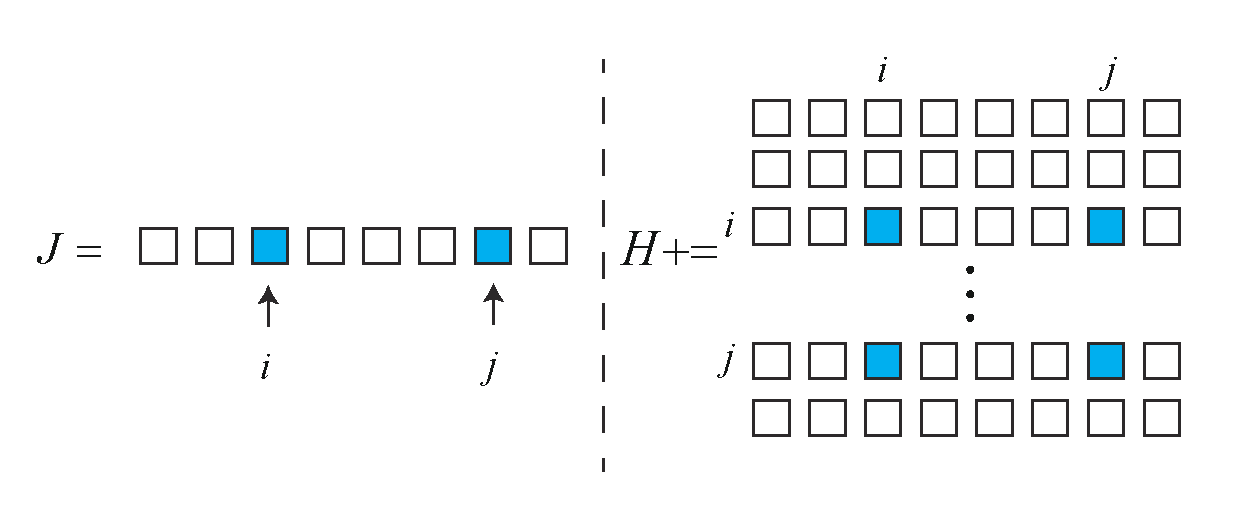
\includegraphics[width=0.3\linewidth]{vo1/sparse}
%    \includegraphics[width=0.3\linewidth]{vo1/semidense}
%    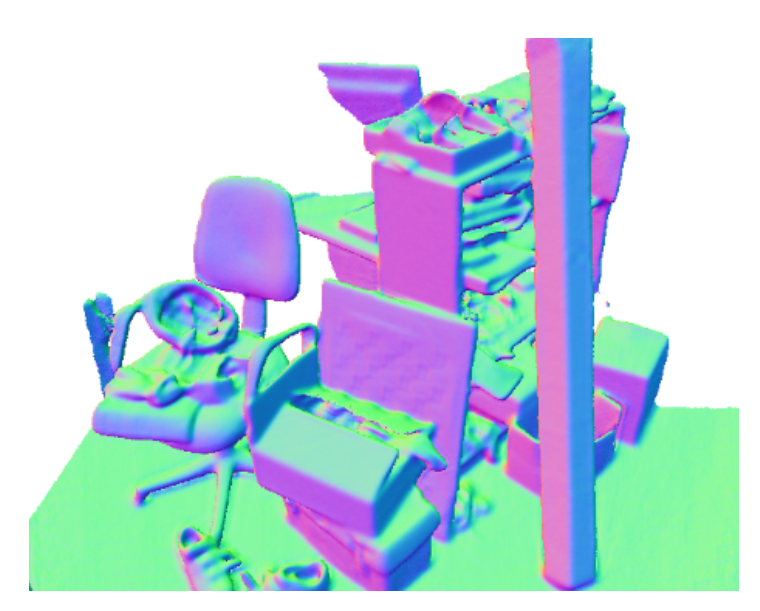
\includegraphics[width=0.3\linewidth]{vo1/dense}
%    \caption{稀疏地图,半稠密地图及稠密地图}
%    \label{fig:threemethods}
%\end{figure}